%%%% https://github.com/jgm/pandoc/blob/master/data/templates/default.latex
% Options for packages loaded elsewhere
\PassOptionsToPackage{unicode}{hyperref}
\PassOptionsToPackage{hyphens}{url}
\PassOptionsToPackage{dvipsnames,svgnames,x11names}{xcolor}
%
\documentclass[
  a4paper,
  twoside,
  titlepage,
  12pt]{article}
\usepackage{amsmath,amssymb}
\usepackage{lmodern}
\usepackage{iftex}
\ifPDFTeX
  \usepackage[T1]{fontenc}
  \usepackage[utf8]{inputenc}
  \usepackage{textcomp} % provide euro and other symbols
\else % if luatex or xetex
  \usepackage{unicode-math}
  \defaultfontfeatures{Scale=MatchLowercase}
  \defaultfontfeatures[\rmfamily]{Ligatures=TeX,Scale=1}
\fi
% Use upquote if available, for straight quotes in verbatim environments
\IfFileExists{upquote.sty}{\usepackage{upquote}}{}
\IfFileExists{microtype.sty}{% use microtype if available
  \usepackage[]{microtype}
  \UseMicrotypeSet[protrusion]{basicmath} % disable protrusion for tt fonts
}{}
\makeatletter
\@ifundefined{KOMAClassName}{% if non-KOMA class
  \IfFileExists{parskip.sty}{%
    \usepackage{parskip}
  }{% else
    \setlength{\parindent}{0pt}
    \setlength{\parskip}{6pt plus 2pt minus 1pt}}
}{% if KOMA class
  \KOMAoptions{parskip=half}}
\makeatother
\usepackage{xcolor}
\IfFileExists{xurl.sty}{\usepackage{xurl}}{} % add URL line breaks if available
\IfFileExists{bookmark.sty}{\usepackage{bookmark}}{\usepackage{hyperref}}
\hypersetup{
  pdftitle={Εγχειρίδιο λειτουργίας ηλιοστάτη.},
  pdfauthor={Νάτσης Αθανάσιος},
  colorlinks=true,
  linkcolor={Maroon},
  filecolor={Maroon},
  citecolor={Blue},
  urlcolor={Blue},
  pdfcreator={LaTeX via pandoc}}
\urlstyle{same} % disable monospaced font for URLs
\usepackage{color}
\usepackage{fancyvrb}
\newcommand{\VerbBar}{|}
\newcommand{\VERB}{\Verb[commandchars=\\\{\}]}
\DefineVerbatimEnvironment{Highlighting}{Verbatim}{commandchars=\\\{\}}
% Add ',fontsize=\small' for more characters per line
\usepackage{framed}
\definecolor{shadecolor}{RGB}{248,248,248}
\newenvironment{Shaded}{\begin{snugshade}}{\end{snugshade}}
\newcommand{\AlertTok}[1]{\textcolor[rgb]{0.94,0.16,0.16}{#1}}
\newcommand{\AnnotationTok}[1]{\textcolor[rgb]{0.56,0.35,0.01}{\textbf{\textit{#1}}}}
\newcommand{\AttributeTok}[1]{\textcolor[rgb]{0.77,0.63,0.00}{#1}}
\newcommand{\BaseNTok}[1]{\textcolor[rgb]{0.00,0.00,0.81}{#1}}
\newcommand{\BuiltInTok}[1]{#1}
\newcommand{\CharTok}[1]{\textcolor[rgb]{0.31,0.60,0.02}{#1}}
\newcommand{\CommentTok}[1]{\textcolor[rgb]{0.56,0.35,0.01}{\textit{#1}}}
\newcommand{\CommentVarTok}[1]{\textcolor[rgb]{0.56,0.35,0.01}{\textbf{\textit{#1}}}}
\newcommand{\ConstantTok}[1]{\textcolor[rgb]{0.00,0.00,0.00}{#1}}
\newcommand{\ControlFlowTok}[1]{\textcolor[rgb]{0.13,0.29,0.53}{\textbf{#1}}}
\newcommand{\DataTypeTok}[1]{\textcolor[rgb]{0.13,0.29,0.53}{#1}}
\newcommand{\DecValTok}[1]{\textcolor[rgb]{0.00,0.00,0.81}{#1}}
\newcommand{\DocumentationTok}[1]{\textcolor[rgb]{0.56,0.35,0.01}{\textbf{\textit{#1}}}}
\newcommand{\ErrorTok}[1]{\textcolor[rgb]{0.64,0.00,0.00}{\textbf{#1}}}
\newcommand{\ExtensionTok}[1]{#1}
\newcommand{\FloatTok}[1]{\textcolor[rgb]{0.00,0.00,0.81}{#1}}
\newcommand{\FunctionTok}[1]{\textcolor[rgb]{0.00,0.00,0.00}{#1}}
\newcommand{\ImportTok}[1]{#1}
\newcommand{\InformationTok}[1]{\textcolor[rgb]{0.56,0.35,0.01}{\textbf{\textit{#1}}}}
\newcommand{\KeywordTok}[1]{\textcolor[rgb]{0.13,0.29,0.53}{\textbf{#1}}}
\newcommand{\NormalTok}[1]{#1}
\newcommand{\OperatorTok}[1]{\textcolor[rgb]{0.81,0.36,0.00}{\textbf{#1}}}
\newcommand{\OtherTok}[1]{\textcolor[rgb]{0.56,0.35,0.01}{#1}}
\newcommand{\PreprocessorTok}[1]{\textcolor[rgb]{0.56,0.35,0.01}{\textit{#1}}}
\newcommand{\RegionMarkerTok}[1]{#1}
\newcommand{\SpecialCharTok}[1]{\textcolor[rgb]{0.00,0.00,0.00}{#1}}
\newcommand{\SpecialStringTok}[1]{\textcolor[rgb]{0.31,0.60,0.02}{#1}}
\newcommand{\StringTok}[1]{\textcolor[rgb]{0.31,0.60,0.02}{#1}}
\newcommand{\VariableTok}[1]{\textcolor[rgb]{0.00,0.00,0.00}{#1}}
\newcommand{\VerbatimStringTok}[1]{\textcolor[rgb]{0.31,0.60,0.02}{#1}}
\newcommand{\WarningTok}[1]{\textcolor[rgb]{0.56,0.35,0.01}{\textbf{\textit{#1}}}}
\usepackage{longtable,booktabs,array}
\usepackage{calc} % for calculating minipage widths
% Correct order of tables after \paragraph or \subparagraph
\usepackage{etoolbox}
\makeatletter
\patchcmd\longtable{\par}{\if@noskipsec\mbox{}\fi\par}{}{}
\makeatother
% Allow footnotes in longtable head/foot
\IfFileExists{footnotehyper.sty}{\usepackage{footnotehyper}}{\usepackage{footnote}}
\makesavenoteenv{longtable}
\setlength{\emergencystretch}{3em} % prevent overfull lines
\providecommand{\tightlist}{%
  \setlength{\itemsep}{0pt}\setlength{\parskip}{0pt}}
\setcounter{secnumdepth}{5}
% \documentclass[a4paper,twoside,titlepage,12pt]{article}

\usepackage{booktabs}
\usepackage{amsthm}

\usepackage{fontspec}
\usepackage{xunicode}
\usepackage{xltxtra}
% \usepackage{xgreek}



\makeatletter
\def\thm@space@setup{%
  \thm@preskip=8pt plus 2pt minus 4pt
  \thm@postskip=\thm@preskip
}
\makeatother
{}

% \usepackage{tabu}

%%%% FONTS
\usepackage{setspace}  % multiple line spaces available
\setstretch{1.3} % maybe need for caption spacing
\setmainfont[Scale=1.1]{Linux Libertine O}  % vv good


%%%% CAPTION  format floats title
\usepackage{caption}
\clearcaptionsetup{}
\captionsetup{justification=justified,
    font={footnotesize},
    singlelinecheck=false,
    width=.85\textwidth,
    labelfont=bf,textfont=it}

%%%% SIUNITX   values and units
\usepackage{siunitx}
\sisetup{mode=text,range-phrase={~με~}}
%\sisetup{range-units=single}
\DeclareSIUnit\decaetia{δεκαετία}
% \sisetup{output-decimal-marker = {,}}
\sisetup{output-decimal-marker = {.}}
\sisetup{expproduct=cdot}
\sisetup{separate-uncertainty = true}

%%%% παράγραφοι noindent και newline
\parskip = \baselineskip


%%%% PAGE GEOMETRY
\usepackage{geometry}
\geometry{
    a4paper,
    left     = 25mm,
    right    = 25mm,
    top      = 30mm,
    bottom   = 30mm,
    headsep  = 3\baselineskip,
    footskip = 4\baselineskip}


%%%% FLOATS
\numberwithin{equation}{section}
\numberwithin{figure}{section}
\numberwithin{table}{section}
\usepackage{float}
\floatstyle{plain}
\floatplacement{figure}{h}
% % \newfloat{img}{htb}{fpic}[section]
% % \newfloat{img}{H}{fpic}[section]
\newfloat{img}{h}{fpic}[section]
\floatname{img}{Εικόνα}


\ifLuaTeX
  \usepackage{selnolig}  % disable illegal ligatures
\fi
\usepackage[]{natbib}
\bibliographystyle{plainnat}

\title{Εγχειρίδιο λειτουργίας ηλιοστάτη.}
\author{Νάτσης Αθανάσιος}
\date{2022-09-30}

\begin{document}
%\maketitle
\begin{titlepage}
    \clearpage\thispagestyle{empty}
    \newlength{\drop} % Command for generating a specific amount of whitespace
    \drop=0.1\textheight % Define the command as 10% of the total text height

    \rule{\textwidth}{1pt}\par % Thick horizontal line
    \vspace{2pt}\vspace{-\baselineskip} % Whitespace between lines
    \rule{\textwidth}{0.4pt}\par % Thin horizontal line

    \vspace{0.6\drop} % Whitespace between the top lines and title
    \centering % Center all text
    %\textcolor{Red}{ % Red font color
        {\Huge  Εγχειρίδιο λειτουργίας ηλιοστάτη,}\\[0.5\baselineskip] % Title line 1
        {\Large Εργαστηρίου Φυσικής της Ατμόσφαιρας.}\\[0.75\baselineskip] % Title line 2
        {\Huge  Sun tracker manual, LAP.} %} % Title line 3

    \vfill
    % \vspace{0.5\drop} % Whitespace between the title and short horizontal line
    % \rule{0.3\textwidth}{0.4pt}\par % Short horizontal line under the title
    % \vspace{\drop} % Whitespace between the thin horizontal line and the author name


\includegraphics[width=0.4\textwidth]{/home/athan/Media/LOGO/LAP3.jpg}

    \vfill

    {\Large Νάτσης Αθανάσιος} \\
    {\small\texttt{natsisthanasis@gmail.com}}\\
    \vspace{10pt}
    {\Large Καραγκιοζίδης Δημήτριος}\\
    {\small\texttt{dkaragki@auth.gr}}\\

    \vfill % Whitespace between the author name and publisher text


    {Θεσσαλονίκη}\\
    {\large \textsc{\the\year-\the\month-\the\day}}\par % Publisher

    % \vspace*{\drop} % Whitespace under the publisher text

    \vfill


    {\small{Ηλεκτρονική έκδοση:} \large\texttt{\href{https://lap-tracker-manual-thanasisn.netlify.app}{lap-tracker-manual-thanasisn.netlify.app}}}\\

    \rule{\textwidth}{0.4pt}\par % Thin horizontal line
    \vspace{2pt}\vspace{-\baselineskip} % Whitespace between lines
    \rule{\textwidth}{1pt}\par % Thick horizontal line
\end{titlepage}
\newpage

% \begin{titlepage}
% \clearpage\thispagestyle{empty}
%     \vspace*{9em}{\centering\Huge\usefont{T1}{qzc}{m}{it}
% Dixie dancing ducks\par}
% \vspace{1em}
% {\hfill\itshape A story of love, hate and fame}
% \clearpage
%     \vspace*{\fill}\hfill   \parbox{.4\textwidth}{
%     \raggedleft
% \scriptsize Delilah was a sad duck with a dream, being a
%     Dixie dancer some day. She wasn't the best looking duck
%     in town but she never cared about superficial things.
%     Practicing a lot she finally became a professional Dixie
%     dancer. She even fell in love. Will Delilah overcome the
%     infamy and hate of her \emph{new gained friends}?
% }
% \end{titlepage}
%
% {\LARGE HEEEEEEEEEEEEEEEEEEEEEELLLLLLLLLLLLLLLLLLLLLLLLLLLOOOEEEEEe}

{
\hypersetup{linkcolor=}
\setcounter{tocdepth}{3}
\tableofcontents
}
\listoffigures
\listoftables
\newpage

\hypertarget{section}{%
\section*{}\label{section}}
\addcontentsline{toc}{section}{}

~

~
\vfill
~

~

\begin{longtable}[]{@{}c@{}}
\toprule()
\endhead
Η εργασία αυτή διανέμεται υπό την άδεια: \\
\textbf{Creative Commons - Αναφορά Δημιουργού -} \\
\textbf{Μη Εμπορική Χρήση - Παρόμοια Διανομή 4.0 Διεθνές.} \\
\url{http://creativecommons.org/licenses/by-nc-sa/4.0/} \\
\bottomrule()
\end{longtable}

~
\vfill ~
~

~
\vfill ~
~

\textbf{\emph{Σημείωση:} Ο πηγαίος κώδικας (source code) που παρατίθεται εδώ είναι ένα παράδειγμα εφαρμογής κάποιων τεχνικών. Σε περίπτωση που θέλετε να τον χρησιμοποιήσετε, προτείνουμε να δοκιμαστεί η καταλληλότητα του για την επιθυμητή χρήση, πρώτα σε μη σημαντικές εφαρμογές (non-critical). Τα παραδείγματα κώδικα εδώ, διαφέρουν από αυτά που χρησιμοποιούμε, λόγω της συνεχής εξέλιξης και βελτίωσης κατά την χρήση τους.}

\newpage

~\\
\vfill
~\\

\hypertarget{intro}{%
\section*{Εισαγωγή.}\label{intro}}
\addcontentsline{toc}{section}{Εισαγωγή.}

Το παρόν είναι ένας ανεπίσημος οδηγός για τη χρήση και τη λειτουργία του ηλιοστάτη του ΕΦΑ. Συντάχτηκε από της διαθέσιμες πληροφορίες για τον ηλιοστάτη καθώς και από την εμπειρία που αποκομίσαμε κατά τη χρήση του. Σκοπός μας είναι να βοηθήσει στην περαιτέρω ανάπτυξη και χρήση του, γι' αυτό ζητούμε την συνεισφορά σας στη βελτίωσή του. Για διορθώσεις και προσθήκες μπορείτε να επικοινωνήσετε με τον \href{mailto:natsisthanasis@gmail.com}{Νάτση Αθανάσιο} (\href{mailto:natsisthanasis@gmail.com}{\nolinkurl{natsisthanasis@gmail.com}}) ή το Εργαστήριο Φυσικής της Ατμόσφαιρας του Α.Π.Θ.

~\\
\vfill
~\\

\newpage

\hypertarget{tracker}{%
\section{Ο ηλιοστάτης του Εργαστηρίου Φυσικής της Ατμόσφαιρας.}\label{tracker}}

\hypertarget{trackerdescription}{%
\subsection{Περιγραφή tracker (ηλιοστάτη).}\label{trackerdescription}}

Η συσκευή αποτελείται από σώμα αλουμινίου, δύο άξονες κίνησης, δύο κινητήρες και ηλεκτρονικό σύστημα ελέγχου.
Οι άξονες έχουν ομόκεντρα γρανάζια τα οποία τίθενται σε κίνηση από stepper motors μέσω κατάλληλου ιμάντα (Εικόνα \ref{fig:trackerinside}).
Η επικοινωνία με το σύστημα ελέγχου γίνεται μέσω σειριακής θύρας (πραγματικής ή εικονικής με τη χρήση μετατροπέα usb/serial).

Και οι δύο κάθετοι άξονες (αζιμούθιου και ζενίθ) έχουν τις ίδιες δυνατότητες και χαρακτηριστικά μεταξύ τους, η λειτουργία τους είναι πανομοιότυπη και μπορούν να κινηθούν ταυτόχρονα και ανεξάρτητα ο ένας από τον άλλο.

Οι κινητήρες του tracker μπορούν να κινηθούν με σταθερό βήμα \(0.6^\circ\) ο καθένας.
Στο πρώτο μοντέλο του ηλιοστάτη, για τη μετάδοση της κίνησης, οι κινητήρες έχουν στο γρανάζι τους 12 δόντια και κινούν μέσω ιμάντα τους άξονες, που έχουν από 70 δόντια ο καθένας.
Αυτό δίνει την δυνατότητα οι άξονες του ηλιοστάτη να κινούνται με διακριτό βήμα \(0.6^\circ \cdot 12 / 70 \simeq 0.10286^\circ\) για το παλιό μοντέλο. Τα καινούρια μοντέλα του ηλιοστάτη, αντίστοιχα έχουν βήμα \({0.125}^\circ\).

Για την εκτέλεση μιας πλήρους περιστροφής του κάθε άξονα ο κινητήρας πρέπει να κάνει \(360^\circ / (0.6^\circ \cdot 12 / 70) = 3500\) βήματα στο παλιό μοντέλο και \(360^\circ / {0.125}^\circ = 2880\) βήματα στα καινούρια μοντέλα.
Ενώ η μέγιστη ταχύτατα περιστροφής των κινητήρων είναι περίπου μία περιστροφή ανά \(15\) δευτερόλεπτα.

\begin{img}

{\centering \includegraphics[width=0.5\linewidth]{../../Aerosols/Photos/EL/20160615_Tracker2/20160615_125806} 

}

\caption{Εσωτερικό του πρώτου μοντέλου tracker. Φαίνονται τα κύρια γρανάζια των αξόνων, ο κινητήρας του αζιμούθιου άξονα και το ηλεκτρονικό σύστημα ελέγχου, καθώς και το CHP 1.}\label{fig:trackerinside}
\end{img}

\hypertarget{tracker_communication}{%
\subsection{Επικοινωνία με τον tracker.}\label{tracker_communication}}

Οι κινητήρες ελέγχονται από μικροελεγκτή (microcontroller), ο οποίος βρίσκεται μέσα στο κύριο σώμα της συσκευής. Ο μικροελεγκτής είναι ήδη προγραμματισμένος να εκτελεί άμεσα τις εντολές που λαμβάνει, μέσω της σειριακής επικοινωνίας.

Το λειτουργικό σύστημα του υπολογιστή αναγνωρίζει τη σειριακή σύνδεση με τον microcontroller ως κάποια θύρα \texttt{COM\#} στα Windows ή ως \texttt{/dev/ttyUSB\#}, \texttt{/dev/ttyS\#} σε GNU/Linux. Οι εντολές μεταδίδονται στη συσκευή, γράφοντάς τις σε κάποια από αυτές τις διευθύνσεις. Αντίστοιχα, οι απαντήσεις των εντολών διαβάζονται από την ίδια διεύθυνση. Τυπικά, η επικοινωνία είναι πανομοιότυπη με την εγγραφή (write) και την ανάγνωση (read) κειμένου (string) από αρχείο, με βήμα, μία γραμμή ανά εντολή. Κάθε γραμμή τερματίζεται με τον χαρακτήρα \texttt{\textquotesingle{}\textbackslash{}r\textquotesingle{}} (Carriage return, CR).

Η σειριακή επικοινωνία μπορεί να επιτευχθεί με άμεση σύνδεση του μικροελεγκτή σε σειριακή θύρα του υπολογιστή. Είτε, μέσω μετατροπέα USB UART (adapter usb to serial) σε θύρα USB του ηλεκτρονικού υπολογιστή (Σχήμα \ref{fig:trackercon}). Στην περίπτωσή μας χρησιμοποιούμε τον μετατροπέα `FT232 USB-Serial (UART) IC'. Υπάρχει το ενδεχόμενο κάποιοι μετατροπείς UART να μην επιτυγχάνουν σωστή επικοινωνία, λόγω των τεχνικών τους χαρακτηριστικών.

\begin{figure}

{\centering 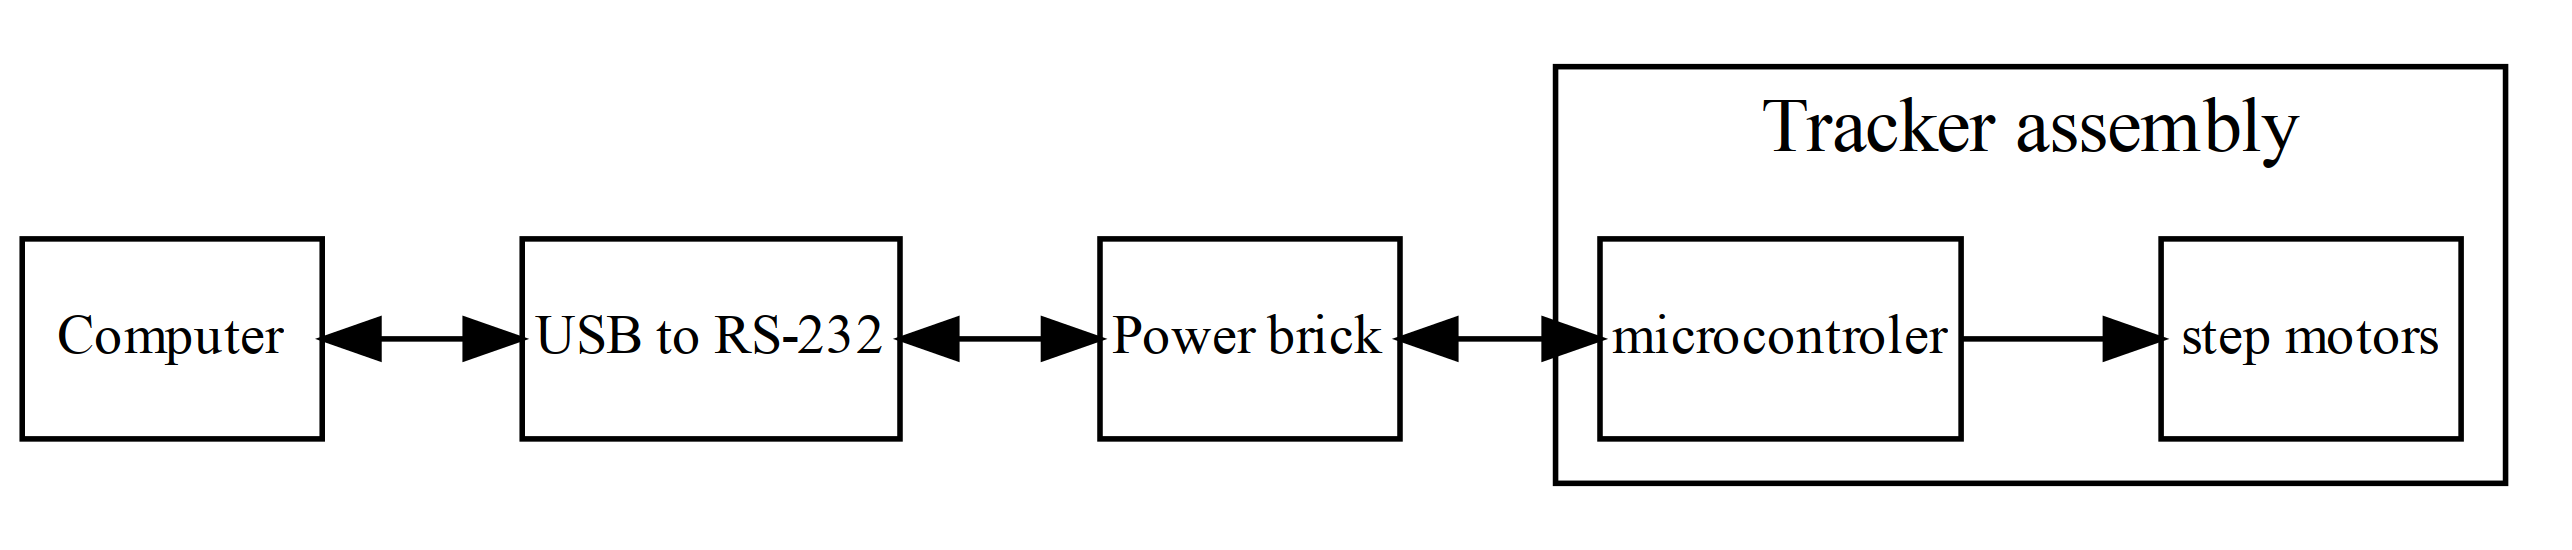
\includegraphics[width=0.8\linewidth]{figure/trackercon} 

}

\caption{Διάγραμμα επικοινωνίας του tracker με τον υπολογιστή.}\label{fig:trackercon}
\end{figure}

\hypertarget{tracker_matlab}{%
\subsubsection{Επικοινωνία με τον Tracker σε περιβάλλον MatLab}\label{tracker_matlab}}

Σε αυτό το στάδιο περιγράφονται οι εντολές και οι παράμετροι που απαιτούνται προκειμένου να επιτευχθεί επικοινωνία με τον Tracker σε περιβάλλον MatLab. Το MatLab διαθέτει έτοιμες συναρτήσεις και εντολές για την επικοινωνία με ένα Serial Object, με την προϋπόθεση να έχουμε εγκατεστημένο το Instrument Control Toolbox. Προτού ανοίξουμε την σειριακή θύρα, πρέπει να δημιουργηθεί ένα Serial Object χρησιμοποιώντας την εντολή \texttt{serial}, εισάγοντας τις αντίστοιχες ρυθμίσεις του Tracker. Στο MatLab snippet που ακολουθεί, ορίζεται μια struct με όνομα `Tracker', η οποία περιλαμβάνει τόσο τις ρυθμίσεις της σειριακής επικοινωνίας (SerialConfiguration), όσο και αυτό καθαυτό το Serial Object (SerialPort). Σημειώνεται ότι στον συγκεκριμένο κώδικα έχει γίνει hard coding της Communication Port σε \texttt{COM4}, καθώς ξέρουμε ότι σε αυτήν την θύρα είναι συνδεδεμένο το καλώδιο USB του Tracker. Για την αυτόματη εύρεση της COM Port μπορεί να χρησιμοποιηθεί η εντολή \texttt{instrfindall} που εντοπίζει όλες τις ενεργές συνδέσεις και επιστρέφει τις θύρες COM, στις οποίες βρίσκονται συνδεδεμένες συσκευές.

\begin{Shaded}
\begin{Highlighting}[]
\CommentTok{\% Set Tracker\textquotesingle{}s Serial Port Configuration and create the Serial Object}
\VariableTok{Tracker}\NormalTok{.}\VariableTok{SerialConfiguration}\NormalTok{.}\VariableTok{COM}             \OperatorTok{=} \SpecialStringTok{\textquotesingle{}COM4\textquotesingle{}}\OperatorTok{;}
\VariableTok{Tracker}\NormalTok{.}\VariableTok{SerialConfiguration}\NormalTok{.}\VariableTok{BaudRate}        \OperatorTok{=} \FloatTok{4800}\OperatorTok{;}
\VariableTok{Tracker}\NormalTok{.}\VariableTok{SerialConfiguration}\NormalTok{.}\VariableTok{DataBit}         \OperatorTok{=} \FloatTok{8}\OperatorTok{;}
\VariableTok{Tracker}\NormalTok{.}\VariableTok{SerialConfiguration}\NormalTok{.}\VariableTok{StopBit}         \OperatorTok{=} \FloatTok{1}\OperatorTok{;}
\VariableTok{Tracker}\NormalTok{.}\VariableTok{SerialConfiguration}\NormalTok{.}\VariableTok{Parity}          \OperatorTok{=} \SpecialStringTok{\textquotesingle{}none\textquotesingle{}}\OperatorTok{;}
\VariableTok{Tracker}\NormalTok{.}\VariableTok{SerialConfiguration}\NormalTok{.}\VariableTok{Terminator}      \OperatorTok{=} \SpecialStringTok{\textquotesingle{}CR\textquotesingle{}}\OperatorTok{;}
\VariableTok{Tracker}\NormalTok{.}\VariableTok{SerialConfiguration}\NormalTok{.}\VariableTok{Timeout}         \OperatorTok{=} \FloatTok{50}\OperatorTok{;}
\VariableTok{Tracker}\NormalTok{.}\VariableTok{SerialConfiguration}\NormalTok{.}\VariableTok{InputBufferSize} \OperatorTok{=} \FloatTok{5000}\OperatorTok{;}

\VariableTok{Tracker}\NormalTok{.}\VariableTok{SerialPort} \OperatorTok{=} \VariableTok{serial}\NormalTok{(}\VariableTok{Tracker}\NormalTok{.}\VariableTok{SerialConfiguration}\NormalTok{.}\VariableTok{COM}\OperatorTok{,...}
    \SpecialStringTok{\textquotesingle{}BaudRate\textquotesingle{}}\OperatorTok{,}\VariableTok{Tracker}\NormalTok{.}\VariableTok{SerialConfiguration}\NormalTok{.}\VariableTok{BaudRate}\OperatorTok{,...}
    \SpecialStringTok{\textquotesingle{}DataBit\textquotesingle{}}\OperatorTok{,}\VariableTok{Tracker}\NormalTok{.}\VariableTok{SerialConfiguration}\NormalTok{.}\VariableTok{DataBit}\OperatorTok{,} \OperatorTok{...}
    \SpecialStringTok{\textquotesingle{}StopBit\textquotesingle{}}\OperatorTok{,}\VariableTok{Tracker}\NormalTok{.}\VariableTok{SerialConfiguration}\NormalTok{.}\VariableTok{StopBit}\OperatorTok{,} \OperatorTok{...}
    \SpecialStringTok{\textquotesingle{}Parity\textquotesingle{}}\OperatorTok{,}\VariableTok{Tracker}\NormalTok{.}\VariableTok{SerialConfiguration}\NormalTok{.}\VariableTok{Parity}\OperatorTok{,} \OperatorTok{...}
    \SpecialStringTok{\textquotesingle{}Terminator\textquotesingle{}}\OperatorTok{,}\VariableTok{Tracker}\NormalTok{.}\VariableTok{SerialConfiguration}\NormalTok{.}\VariableTok{Terminator}\OperatorTok{,} \OperatorTok{...}
    \SpecialStringTok{\textquotesingle{}Timeout\textquotesingle{}}\OperatorTok{,}\VariableTok{Tracker}\NormalTok{.}\VariableTok{SerialConfiguration}\NormalTok{.}\VariableTok{Timeout}\OperatorTok{,} \OperatorTok{...}
    \SpecialStringTok{\textquotesingle{}InputBufferSize\textquotesingle{}}\OperatorTok{,}\VariableTok{Tracker}\NormalTok{.}\VariableTok{SerialConfiguration}\NormalTok{.}\VariableTok{InputBufferSize}\NormalTok{)}\OperatorTok{;}
\end{Highlighting}
\end{Shaded}

Η παράμετρος \texttt{InputBufferSize} επιτρέπει τον έλεγχο του αριθμού των bytes που μπορούν να κρατηθούν στον buffer του μικροεπεξεργαστή και εφόσον δοθεί μια μεγάλη τιμή (όπως στην περίπτωσή μας, 5000), μπορούμε να δίνουμε εντολές στον Tracker την μία πίσω από την άλλη σε stack. Υπόψιν ότι ο μικροεπεξεργαστής σε αυτήν την περίπτωση θα επιστρέψει ως πρώτη απάντηση το αποτέλεσμα της εντολής που ολοκληρώθηκε πρώτη και στην συνέχεια με την ίδια λογική τις υπόλοιπες. Αφού δημιουργηθεί το Serial Object, χρησιμοποιώντας τις εντολές \texttt{fopen} και \texttt{fclose} μπορούμε να ανοίξουμε και να κλείσουμε αντίστοιχα την σειριακή θύρα. Με τις εντολές \texttt{fprintf} και \texttt{fscanf} δίνουμε εντολή στον Tracker και λαμβάνουμε την απάντησή του αντίστοιχα σε μορφή ASCII. Παρακάτω παρουσιάζεται ένα παράδειγμα για την εύρεση της θέσης (step) του Αζιμούθιου άξονα

\begin{Shaded}
\begin{Highlighting}[]
\CommentTok{\% Send the Command to the Tracker}
\VariableTok{fprintf}\NormalTok{(}\VariableTok{Tracker}\NormalTok{.}\VariableTok{SerialPort}\OperatorTok{,} \SpecialStringTok{\textquotesingle{}AZ?\textquotesingle{}}\NormalTok{)}\OperatorTok{;}
\end{Highlighting}
\end{Shaded}

\begin{Shaded}
\begin{Highlighting}[]
\CommentTok{\% Wait for the Tracker\textquotesingle{}s microntroller to fill the buffer (Typically 0.5 sec)}
\VariableTok{pause}\NormalTok{(}\VariableTok{time\_delay}\NormalTok{)}
\end{Highlighting}
\end{Shaded}

\begin{Shaded}
\begin{Highlighting}[]
\CommentTok{\% Get the Tracker\textquotesingle{}s answer}
\NormalTok{[}\VariableTok{answer}\OperatorTok{,} \VariableTok{bytes}\OperatorTok{,} \VariableTok{msg\_err}\NormalTok{] }\OperatorTok{=} \VariableTok{fscanf}\NormalTok{(}\VariableTok{Tracker}\NormalTok{.}\VariableTok{SerialPort}\NormalTok{)}\OperatorTok{;}
\end{Highlighting}
\end{Shaded}

Με τις παραπάνω εντολές, ο Tracker θα απαντήσει με την θέση σε βήματα του Αζιμούθιου άξονα (πχ AZ:6000) στην μεταβλητή \texttt{answer}, τον αριθμό των bytes που στάλθηκαν (8 στην συγκεκριμένη περίπτωση) στην μεταβλητή \texttt{bytes} και τυχόν μηνύματα σφάλματος κατά την σειριακή επικοινωνία στην μεταβλητή \texttt{msg\_err}. Άλλες χρήσιμες εντολές και παράμετροι για τον έλεγχο και την ορθή επικοινωνία με τον Tracker είναι η \texttt{Tracker.SerialPort.BytesAvailable}, η οποία επιστρέφει τον αριθμό των bytes που υπάρχουν διαθέσιμα στον buffer του microcontroller, η \texttt{flushinput(Tracker.SerialPort)} και η \texttt{flushoutput(Tracker.SerialPort)} που αδειάζουν τον Input και Output buffer αντίστοιχα.

\hypertarget{tracker_connection}{%
\subsection{Σειρά σύνδεσης.}\label{tracker_connection}}

Μετά από δοκιμές όλων των δυνατών συνδυασμών της σειρά σύνδεσης. Διαπιστώσαμε ότι για την επιτυχή επικοινωνία πρέπει να έχει γίνει η σύνδεση (4) και μετά να ακολουθηθεί η σειρά των συνδέσεων (1-2-3) ή (3-2-1) όπως φαίνονται στο Σχήμα \ref{fig:trackercomm}.

\begin{figure}

{\centering 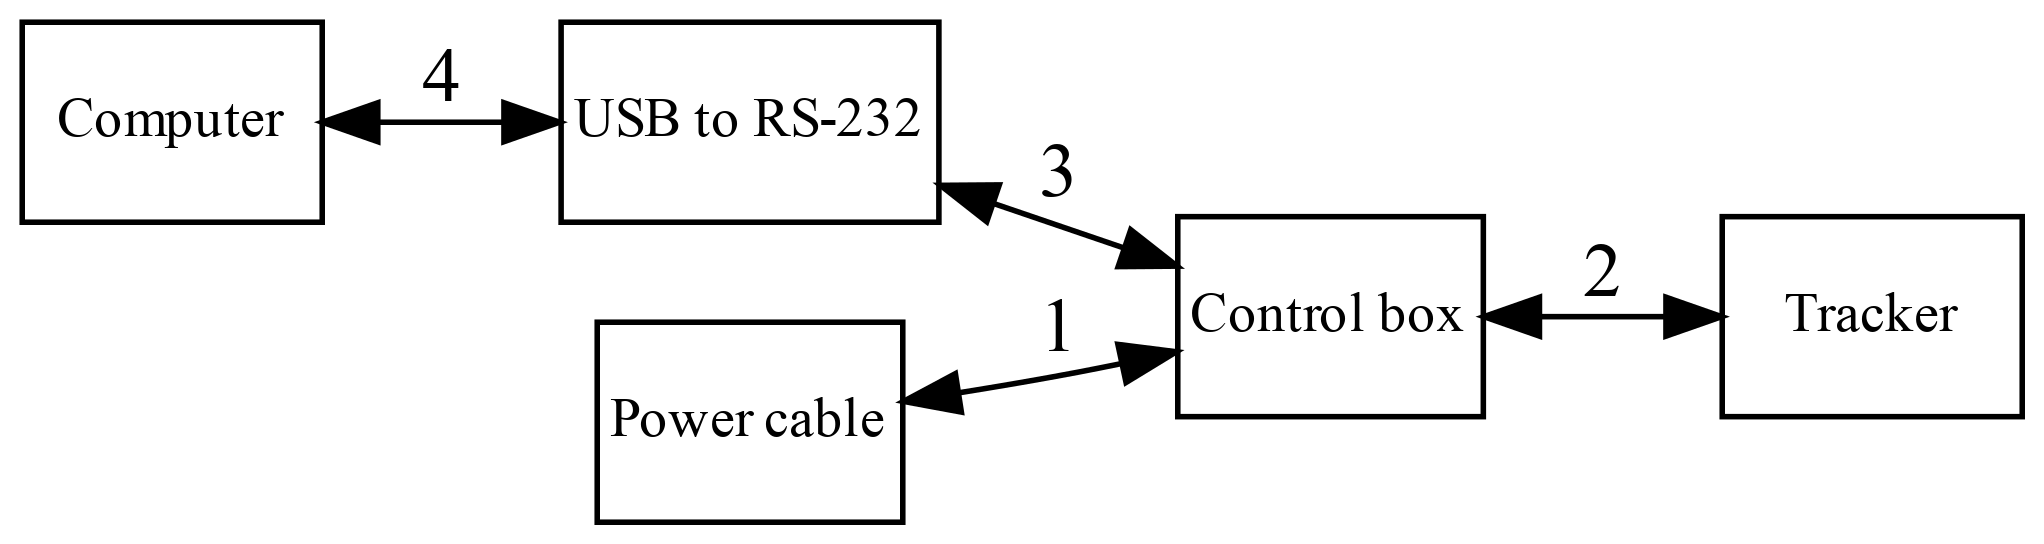
\includegraphics[width=0.8\linewidth]{figure/trackercomm} 

}

\caption{Διάγραμμα συνδέσεων του tracker, κατάλληλη σειρά σύνδεσης (1-2-3) ή (3-2-1).}\label{fig:trackercomm}
\end{figure}

\newpage

\hypertarget{trackeroperation}{%
\section{Λειτουργία - Προγραμματισμός tracker.}\label{trackeroperation}}

\hypertarget{ux3b3ux3b5ux3bdux3b9ux3baux3adux3c2-ux3c0ux3bbux3b7ux3c1ux3bfux3c6ux3bfux3c1ux3afux3b5ux3c2}{%
\subsection{Γενικές πληροφορίες}\label{ux3b3ux3b5ux3bdux3b9ux3baux3adux3c2-ux3c0ux3bbux3b7ux3c1ux3bfux3c6ux3bfux3c1ux3afux3b5ux3c2}}

Κατά τη λειτουργία πρέπει να δοθεί προσοχή, διότι δεν υπάρχει μηχανικός περιορισμός που να αποτρέπει την περιστροφή του άξονα κατά γωνίες μεγαλύτερες του πλήρη κύκλου.
Αυτό μπορεί να προκαλέσει πρόβλημα γιατί το καλώδιο του tracker αλλά και τον οργάνων μπορεί να τυλιχτούν γύρω από τον άξονα και να καταστραφούν.
Επίσης, σε περίπτωση που η συσκευή δεν έχει τοποθετηθεί μόνιμα π.χ. σε τρίποδα, μπορεί η περιστροφή να τραβήξει τα καλώδια και να ρίξει τη συσκευή.

Ο tracker όταν του δοθεί εντολή (reset), θα προσπαθήσει να μηδενίσει τον μετρητή βήματος αφού μετακινηθεί σε μία γνωστή θέση.
Αυτό γίνεται με την περιστροφή του άξονα, μέχρι να φτάσει στη συγκεκριμένη θέση, την οποία αναγνωρίζει με μία φωτοδίοδο.
Προσοχή, σε περίπτωση που δεν πάρει σήμα από τη φωτοδίοδο, θα συνεχίσει να περιστρέφεται ασταμάτητα.
Αυτό μπορεί να συμβεί, αν το καπάκι είναι ανοιχτό σε έντονο φως ή αν υπάρχει κάποιο πρόβλημα επικοινωνίας με τη φωτοδίοδο.

Ο tracker θα μηδενίσει τον κάθε άξονα στη θέση \texttt{\textquotesingle{}5000\textquotesingle{}}. Από εκεί και πέρα μπορεί να κινηθεί και προς τις δύο κατευθύνσεις.
Προσοχή, αν το βήμα γίνει αρνητικό από κάποια εντολή ή αν γίνει μεγαλύτερο του \texttt{\textquotesingle{}9999\textquotesingle{}} ο tracker θα κολλήσει και θα συνεχίσει να περιστρέφεται ασταμάτητα.
Αυτό πρέπει να αποφευχθεί μέσω του προγραμματισμού του. Μελλοντικά μπορεί να προστεθεί κάποιος μηχανικός ή ηλεκτρικός μηχανισμός περιορισμού.

Εάν το βήμα γίνει ακατάλληλο και ο tracker περιστρέφεται ασταμάτητα, μπορεί να σταματήσει με την εντολή \texttt{\textquotesingle{}stop\textquotesingle{}}.
Σε αυτήν την περίπτωση, αν ερωτηθεί για τη θέση του επιστρέφει την τιμή \texttt{\textquotesingle{}9999\textquotesingle{}}.

Όταν ο ηλιοστάτης τροφοδοτείται και είναι σε λειτουργία, οι κινητήρες δεν θα επιτρέψουν την ελεύθερη περιστροφή των αξόνων.
Σε περίπτωση που χρειάζεται να περιστραφούν ελεύθερα, πρέπει να διακοπεί η τροφοδοσία. \textbf{Σημείωση}: για το πρώτο/παλιό μοντέλο του ηλιοστάτη (ορθογώνιο παραλληλόγραμμο καπάκι) η αντίσταση των κινητήρων σε εξωτερική περιστροφή είναι πολύ μικρή, με αποτέλεσμα να είναι εύκολη η τυχαία μετατόπισή του από εξωτερικούς παράγοντες.
Σε αυτή την περίπτωση, είναι καλό να γίνει επανεκκίνηση του προγράμματος ελέγχου του tracker, ώστε να ξαναβρεί τη θέση του κάνοντας reset των αξόνων και στην συνέχεια, να ελεγχθεί αν η διόπτευση (sighting) συνεχίζει να είναι σωστή.

\hypertarget{ux3c0ux3b1ux3c1ux3acux3bcux3b5ux3c4ux3c1ux3bfux3b9-ux3b5ux3c0ux3b9ux3baux3bfux3b9ux3bdux3c9ux3bdux3afux3b1ux3c2-ux3bcux3b5-ux3c4ux3bfux3bd-microcontroller-ux3c4ux3bfux3c5-tracker.}{%
\subsection{Παράμετροι επικοινωνίας με τον microcontroller του tracker.}\label{ux3c0ux3b1ux3c1ux3acux3bcux3b5ux3c4ux3c1ux3bfux3b9-ux3b5ux3c0ux3b9ux3baux3bfux3b9ux3bdux3c9ux3bdux3afux3b1ux3c2-ux3bcux3b5-ux3c4ux3bfux3bd-microcontroller-ux3c4ux3bfux3c5-tracker.}}

Στον Πίνακα \ref{tab:trackerserial} περιγράφονται οι απαραίτητες παράμετροι για την σύνδεση με τη σειριακή θύρα του tracker. Κατά την επικοινωνία, είναι χρήσιμο να υπάρχει και κάποιο άνω όριο στον χρόνο που περιμένει ο υπολογιστής, πριν αποφασίσει ότι η επικοινωνία δεν είναι εφικτή. Διαφορετικά, αν κάποιο μήνυμα περιμένει να διαβαστεί από τη θύρα και αυτό δεν γίνει, μπορεί να παγώσει η επικοινωνία.

\footnotesize

\begin{longtable}[]{@{}rl@{}}
\caption{\label{tab:trackerserial} Παράμετροι επικοινωνίας του tracker μέσω σειριακής θύρας RS-232.}\tabularnewline
\toprule()
\endhead
\textbf{bits per second} & \textbf{4800} (baudrate) \\
\textbf{data bits} & \textbf{8} (bytesize) \\
\textbf{parity} & \textbf{none} \\
\textbf{stop bits} & \textbf{1} \\
\textbf{row control} & \textbf{none} \\
\textbf{timeout} (optional) & 90 sec \\
\bottomrule()
\end{longtable}

\normalsize

\hypertarget{ux3b5ux3bdux3c4ux3bfux3bbux3adux3c2-tracker.}{%
\subsection{Εντολές tracker.}\label{ux3b5ux3bdux3c4ux3bfux3bbux3adux3c2-tracker.}}

\hypertarget{ux3bcux3bfux3c1ux3c6ux3ae-ux3b5ux3bdux3c4ux3bfux3bbux3ceux3bd-format.}{%
\subsubsection{Μορφή εντολών (format).}\label{ux3bcux3bfux3c1ux3c6ux3ae-ux3b5ux3bdux3c4ux3bfux3bbux3ceux3bd-format.}}

Η επικοινωνία με τον microcontroller του tracker γίνεται με εντολές που στέλνονται μέσω σειριακής θύρας επικοινωνίας. Οι εντολές έχουν την μορφή κειμένου `string' το οποίο τερματίζεται με το σύμβολο \texttt{\textquotesingle{}cr\textquotesingle{}} ή \texttt{\textquotesingle{}\textbackslash{}r\textquotesingle{}} (`carriage return' το τυπικό `enter' των MS Windows).

Οι εντολές που έχουν ως όρισμα αριθμό βημάτων, πρέπει να δίνονται με διαμόρφωση τεσσάρων ψηφίων. Όταν είναι αναγκαίο πρέπει να προπορεύονται από τα αντίστοιχα μηδενικά (padded with zero). Για παράδειγμα 1000, 0999, 0099, 0001. Αυτό ισχύει για την απόλυτη θέση (π.χ. \texttt{\textquotesingle{}AZ=0100\textquotesingle{}}) και για τη σχετική μετατόπιση (\texttt{\textquotesingle{}AZ+0100\textquotesingle{}}).

Αντίστοιχα, οι εντολές που αφορούν ταχύτητες έχουν την ίδια λογική μόνο που χρησιμοποιούν δύο ψηφία.

\textbf{Προσοχή:} Η απάντηση κάθε εντολής (ανάλογα και με τις ρυθμίσεις της σειριακής επικοινωνίας) πρέπει να διαβαστεί από τη σειριακή σύνδεση γιατί διαφορετικά δεν θα αδειάσει το buffer της σειριακής θύρας και μπορεί να παγώσει η επικοινωνία.

\hypertarget{ux3bcux3b7ux3b4ux3b5ux3bdux3b9ux3c3ux3bcux3ccux3c2-ux3c4ux3bfux3c5-ux3b2ux3aeux3bcux3b1ux3c4ux3bfux3c2-ux3c4ux3bfux3c5-microcontroller.}{%
\subsubsection{Μηδενισμός του βήματος του microcontroller.}\label{ux3bcux3b7ux3b4ux3b5ux3bdux3b9ux3c3ux3bcux3ccux3c2-ux3c4ux3bfux3c5-ux3b2ux3aeux3bcux3b1ux3c4ux3bfux3c2-ux3c4ux3bfux3c5-microcontroller.}}

Οι εντολές reset του Πίνακα \ref{tab:trackercomstr} επιστρέφουν τους κινητήρες στην αρχική τους (`μηδενική') θέση.
Ο microcontroller αναλαμβάνει την κίνηση. Τους περιστρέφει μέχρι την φωτοδίοδο και εκεί ρυθμίζει το εσωτερικό βήμα κάθε άξονα στη τιμή \texttt{5000}.
Μετά την εκτέλεση της εντολής ο tracker επιστρέφει τη διαφορά στη θέση από τον προηγούμενο μηδενισμό. Αυτές οι εντολές συνήθως χρησιμοποιούνται κατά την εκκίνηση της λειτουργίας ώστε να βεβαιωθούμε για την απόλυτη θέση του tracker, αφού δεν υπάρχει άλλος μηχανισμός αναγνώρισης της θέσης.
Προσοχή, για την σωστή λειτουργία του μηδενισμού, οι παρακάτω εντολές πρέπει να δοθούν ξεχωριστά (όχι σε stack) και να περιμένουμε τον μηδενισμό του κάθε άξονα με την αντίστοιχη απάντηση από τον Tracker προτού δοθεί η επόμενη εντολή. Έπειτα από τον μηδενισμό του κάθε άξονα πρέπει να δοθεί εντολή κίνησης του ίδιου άξονα πριν δοθεί εντολή μηδενισμού του επόμενου άξονα, αλλιώς δημιουργείται πρόβλημα στην επικοινωνία και ο Tracker στην συνέχεια δεν επιστρέφει την απάντηση OK όταν μεταβεί σε κάποια ζητούμενη θέση. Υποθέτοντας ότι η θέση του αζιμούθιου, του ζενίθ και του φίλτρου της φωτοδιόδου είναι 5000, προτείνεται μετά από τον μηδενισμό του κάθε άξονα η κίνηση του ίδιου άξονα στην θέση 5000 (δεν θα μετακινηθεί αφού ήδη βρίσκεται σε αυτήν την θέση, ωστόσο αποφεύγεται το πρόβλημα της επικοινωνίας).

\footnotesize

\begin{longtable}[]{@{}
  >{\centering\arraybackslash}p{(\columnwidth - 4\tabcolsep) * \real{0.2069}}
  >{\centering\arraybackslash}p{(\columnwidth - 4\tabcolsep) * \real{0.3448}}
  >{\centering\arraybackslash}p{(\columnwidth - 4\tabcolsep) * \real{0.4483}}@{}}
\caption{\label{tab:trackercomstr} Εντολές μηδενισμού (reset) των αξόνων του tracker.}\tabularnewline
\toprule()
\begin{minipage}[b]{\linewidth}\centering
Εντολή
\end{minipage} & \begin{minipage}[b]{\linewidth}\centering
Λειτουργία
\end{minipage} & \begin{minipage}[b]{\linewidth}\centering
Απάντηση tracker
\end{minipage} \\
\midrule()
\endfirsthead
\toprule()
\begin{minipage}[b]{\linewidth}\centering
Εντολή
\end{minipage} & \begin{minipage}[b]{\linewidth}\centering
Λειτουργία
\end{minipage} & \begin{minipage}[b]{\linewidth}\centering
Απάντηση tracker
\end{minipage} \\
\midrule()
\endhead
\textbf{\texttt{DA}}\textless cr\textgreater{} & reset azimuth motor & \texttt{eA:\#\#\#\#} (όταν βρει τη φωτοδίοδο) \\
\textbf{\texttt{DF}}\textless cr\textgreater{} & reset filters (not used) & \texttt{eF:\#\#\#\#} (όταν βρει τη φωτοδίοδο) \\
\textbf{\texttt{DZ}}\textless cr\textgreater{} & reset zenith motor & \texttt{eZ:\#\#\#\#} (όταν βρει τη φωτοδίοδο) \\
\bottomrule()
\end{longtable}

\normalsize

\hypertarget{ux3baux3afux3bdux3b7ux3c3ux3b7-ux3c4ux3c9ux3bd-ux3b1ux3beux3ccux3bdux3c9ux3bd.}{%
\subsubsection{Κίνηση των αξόνων.}\label{ux3baux3afux3bdux3b7ux3c3ux3b7-ux3c4ux3c9ux3bd-ux3b1ux3beux3ccux3bdux3c9ux3bd.}}

Η εντολές για την κίνηση των αξόνων έχουν τρία μέρη και έχουν τη γενική μορφή: \textbf{\texttt{xx@\#\#\#\#\textless{}cr\textgreater{}}}. Η εξήγηση των επιμέρους στοιχείων γίνεται στον Πίνακα \ref{tab:trackercompart} και \ref{tab:trackercomoper}. Παραδείγματα έγκυρων εντολών βρίσκονται στον Πίνακα \ref{tab:trackercomexamp}. Ενώ, το σύνολο των εντολών παρατίθεται στον Πίνακα \ref{tab:trackercommands}.

\footnotesize

\begin{longtable}[]{@{}
  >{\raggedleft\arraybackslash}p{(\columnwidth - 2\tabcolsep) * \real{0.1918}}
  >{\raggedright\arraybackslash}p{(\columnwidth - 2\tabcolsep) * \real{0.8082}}@{}}
\caption{\label{tab:trackercompart} Τα μέρη της εντολής του tracker.}\tabularnewline
\toprule()
\begin{minipage}[b]{\linewidth}\raggedleft
Παράμετρος
\end{minipage} & \begin{minipage}[b]{\linewidth}\raggedright
Λειτουργία
\end{minipage} \\
\midrule()
\endfirsthead
\toprule()
\begin{minipage}[b]{\linewidth}\raggedleft
Παράμετρος
\end{minipage} & \begin{minipage}[b]{\linewidth}\raggedright
Λειτουργία
\end{minipage} \\
\midrule()
\endhead
\textbf{\texttt{xx}} & Η παράμετρος στην οποία αναφέρεται \\
\texttt{@} & Ο modifier της λειτουργίας που εκτελείται ( ?, =, +, - ) \\
\textbf{\texttt{\#\#\#\#}} & Αριθμητική τιμή της εντολής (\#\#: για τις ταχύτητες) \\
\textless cr\textgreater{} & Ο χαρακτήρας τερματισμού της εντολής. \\
\bottomrule()
\end{longtable}

\begin{longtable}[]{@{}
  >{\centering\arraybackslash}p{(\columnwidth - 4\tabcolsep) * \real{0.1495}}
  >{\raggedright\arraybackslash}p{(\columnwidth - 4\tabcolsep) * \real{0.6262}}
  >{\raggedright\arraybackslash}p{(\columnwidth - 4\tabcolsep) * \real{0.2243}}@{}}
\caption{\label{tab:trackercomoper} Παράμετροι ελέγχου (operators/modifiers) εντολών tracker.}\tabularnewline
\toprule()
\begin{minipage}[b]{\linewidth}\centering
Modifier (@)
\end{minipage} & \begin{minipage}[b]{\linewidth}\raggedright
Λειτουργία
\end{minipage} & \begin{minipage}[b]{\linewidth}\raggedright
Απάντηση
\end{minipage} \\
\midrule()
\endfirsthead
\toprule()
\begin{minipage}[b]{\linewidth}\centering
Modifier (@)
\end{minipage} & \begin{minipage}[b]{\linewidth}\raggedright
Λειτουργία
\end{minipage} & \begin{minipage}[b]{\linewidth}\raggedright
Απάντηση
\end{minipage} \\
\midrule()
\endhead
\textbf{\texttt{?}} & Ζητά την τιμή της μεταβλητής από τον tracker (χωρίς \texttt{\#\#\#\#}) & xx:\#\#\#\#\textless cr\textgreater{} ή xx:\#\#\textless cr\textgreater{} για τις παραμέτρους ταχύτητας \\
\textbf{\texttt{=}} & Θέτει την τιμή της μεταβλητής σε αυτήν την τιμή
(\texttt{\#\#} για τις παραμέτρους ταχύτητας και \texttt{\#\#\#\#} για τις
υπόλοιπες παραμέτρους) & OK\textless cr\textgreater{} \\
\textbf{\texttt{+}} & Αυξάνει την τιμή της μεταβλητής κατά τη δοσμένη τιμή
(\texttt{\#\#} για τις παραμέτρους ταχύτητας και \texttt{\#\#\#\#} για τις
υπόλοιπες παραμέτρους) & OK\textless cr\textgreater{} \\
\textbf{\texttt{-}} & Μειώνει την τιμή της μεταβλητής κατά τη δοσμένη τιμή
(\texttt{\#\#} για τις παραμέτρους ταχύτητας και \texttt{\#\#\#\#} για τις
υπόλοιπες παραμέτρους) & OK\textless cr\textgreater{} \\
\bottomrule()
\end{longtable}

\begin{longtable}[]{@{}
  >{\raggedleft\arraybackslash}p{(\columnwidth - 2\tabcolsep) * \real{0.2766}}
  >{\raggedright\arraybackslash}p{(\columnwidth - 2\tabcolsep) * \real{0.7234}}@{}}
\caption{\label{tab:trackercommands} Εντολές tracker.}\tabularnewline
\toprule()
\begin{minipage}[b]{\linewidth}\raggedleft
Εντολές
\end{minipage} & \begin{minipage}[b]{\linewidth}\raggedright
Μέγεθος
\end{minipage} \\
\midrule()
\endfirsthead
\toprule()
\begin{minipage}[b]{\linewidth}\raggedleft
Εντολές
\end{minipage} & \begin{minipage}[b]{\linewidth}\raggedright
Μέγεθος
\end{minipage} \\
\midrule()
\endhead
\textbf{\texttt{AZ@\#\#\#\#}}\textless cr\textgreater{} & Αζιμούθιο βήμα \\
\textbf{ZE@\#\#\#\#}\textless cr\textgreater{} & Ζενίθιο βήμα \\
\textbf{FR@\#\#\#\#}\textless cr\textgreater{} & Βήμα φίλτρου \\
\textbf{SA@\#\#}\textless cr\textgreater{} & Ταχύτητα αζιμούθιου άξονα \\
\textbf{SZ@\#\#}\textless cr\textgreater{} & Ταχύτητα ζενίθιου άξονα \\
\textbf{SF@\#\#}\textless cr\textgreater{} & Ταχύτητα φίλτρου \\
\textbf{OA@\#\#\#\#}\textless cr\textgreater{} & Τροποποίηση αρχικής αζιμούθιας θέσης \\
\textbf{OZ@\#\#\#\#}\textless cr\textgreater{} & Τροποποίηση αρχικής ζενίθιας θέσης \\
\textbf{OF@\#\#\#\#}\textless cr\textgreater{} & Τροποποίηση αρχικής θέσης φίλτρου \\
\textbf{IA@\#\#\#\#}\textless cr\textgreater{} & Τροποποίηση της αζιμούθιας θέσης της φωτοδιόδου \\
\textbf{IZ@\#\#\#\#}\textless cr\textgreater{} & Τροποποίηση της ζενίθιας θέσης της φωτοδιόδου \\
\textbf{IF@\#\#\#\#}\textless cr\textgreater{} & Τροποποίηση της θέσης του φίλτρου της φωτοδιόδου \\
\textbf{TA@\#\#\#\#}\textless cr\textgreater{} & Τροποποίηση της ζητούμενης αζιμούθιας θέσης (μόνο ερώτηση) \\
\textbf{TZ@\#\#\#\#}\textless cr\textgreater{} & Τροποποίηση της ζενίθιας αζιμούθιας θέσης (μόνο ερώτηση) \\
\textbf{TF@\#\#\#\#}\textless cr\textgreater{} & Τροποποίηση της ζητούμενης θέσης του φίλτρου (μόνο ερώτηση) \\
\textbf{GO XXXX,YYYY}\textless cr\textgreater{} & Μετακινεί ταυτόχρονα την αζιμούθια και ζενίθια θέση σε XXXX και YYYY βήματα αντίστοιχα \\
\textbf{STOP}\textless cr\textgreater{} & Σταματά την κίνηση του tracker \\
\textbf{DEBUG ON/OFF}\textless cr\textgreater{} & Toggles debug mode on/off. Στην περίπτωση του ON, ο Tracker επιστρέφει τόσο την εντολή που του δόθηκε, όσο και την αντίστοιχη απάντηση \\
\bottomrule()
\end{longtable}

\normalsize

Η εντολή \textbf{\texttt{stop\textless{}cr\textgreater{}}} σταματά την κίνηση των αξόνων. Λειτουργεί ακόμα και όταν ο tracker έχει `κολλήσει'. Όταν δηλαδή, το βήμα κάποιου άξονα έχει φτάσει σε μη επιτρεπτή τιμή. Σε αυτή τη κατάσταση, ο tracker απαντά την τιμή \texttt{9999} στο ερώτημα της θέσης, ενώ ο άξονας περιστρέφεται ασταμάτητα.

\footnotesize

\begin{longtable}[]{@{}
  >{\centering\arraybackslash}p{(\columnwidth - 2\tabcolsep) * \real{0.2840}}
  >{\raggedright\arraybackslash}p{(\columnwidth - 2\tabcolsep) * \real{0.7160}}@{}}
\caption{\label{tab:trackercomexamp} Παραδείγματα εντολών tracker.}\tabularnewline
\toprule()
\begin{minipage}[b]{\linewidth}\centering
Εντολή
\end{minipage} & \begin{minipage}[b]{\linewidth}\raggedright
Αποτέλεσμα
\end{minipage} \\
\midrule()
\endfirsthead
\toprule()
\begin{minipage}[b]{\linewidth}\centering
Εντολή
\end{minipage} & \begin{minipage}[b]{\linewidth}\raggedright
Αποτέλεσμα
\end{minipage} \\
\midrule()
\endhead
\textbf{AZ=6000}\textless cr\textgreater{} & Αζιμούθιο στη θέση 6000 \\
\textbf{ZE+0010}\textless cr\textgreater{} & Ζενίθ +10 βήματα \\
\textbf{AZ-0100}\textless cr\textgreater{} & Αζιμούθιο -100 βήματα \\
\textbf{AZ?}\textless cr\textgreater{} & Απάντηση: AZ:5900\textless cr\textgreater{} \\
\textbf{SA=60}\textless cr\textgreater{} & Ταχύτητα του αζιμούθιου άξονα 60 \\
\textbf{?}\textless cr\textgreater{} & \begin{minipage}[t]{\linewidth}\raggedright
θέσεις των δύο αξόνων και του φίλτρου.\\
Απάντησεις: AZ:2345\textless cr\textgreater, ZE:5678\textless cr\textgreater, FR:3456\textless cr\textgreater{}\strut
\end{minipage} \\
\bottomrule()
\end{longtable}

\normalsize

\hypertarget{resetting-usbserial-interface-ux3c3ux3b5-gnulinux.}{%
\subsection{Resetting USB/serial interface σε GNU/Linux.}\label{resetting-usbserial-interface-ux3c3ux3b5-gnulinux.}}

Κάποιες ιδέες και προτάσεις για το πως μπορεί να γίνει επανασύνδεση της επικοινωνίας χωρίς να αποσυνδεθεί η φυσική σύνδεση. Έχουν παραχθεί και τα αντίστοιχα `bash script' που μπορούν να βρουν την κατάλληλη USB συσκευή και να εκτελέσουν τις παρακάτω ενέργειες.

\hypertarget{ux3b1ux3c0ux3bfux3c3ux3cdux3bdux3b4ux3b5ux3c3ux3b7-ux3c4ux3c9ux3bd-ux3b1ux3bdux3c4ux3afux3c3ux3c4ux3bfux3b9ux3c7ux3c9ux3bd-modulefirmware-ux3b1ux3c0ux3cc-ux3c4ux3bfux3bd-kernel.}{%
\subsubsection{Αποσύνδεση των αντίστοιχων module/firmware από τον kernel.}\label{ux3b1ux3c0ux3bfux3c3ux3cdux3bdux3b4ux3b5ux3c3ux3b7-ux3c4ux3c9ux3bd-ux3b1ux3bdux3c4ux3afux3c3ux3c4ux3bfux3b9ux3c7ux3c9ux3bd-modulefirmware-ux3b1ux3c0ux3cc-ux3c4ux3bfux3bd-kernel.}}

Αυτές οι εντολές απενεργοποιούν και ενεργοποιούν τα κομμάτια του συστήματος που χειρίζονται τις σειριακές συσκευές και τις συσκευές USB.

\begin{Shaded}
\begin{Highlighting}[]
\ExtensionTok{rmmod}\NormalTok{  ftdi\_sio}
\ExtensionTok{rmmod}\NormalTok{  usbserial}
\ExtensionTok{modprobe}\NormalTok{ ftdi\_sio}
\ExtensionTok{modprobe}\NormalTok{ usbserial}
\end{Highlighting}
\end{Shaded}

\hypertarget{ux3b1ux3c0ux3bfux3c3ux3cdux3bdux3b4ux3b5ux3c3ux3b7-ux3c4ux3b7ux3c2-ux3c3ux3c5ux3c3ux3baux3b5ux3c5ux3aeux3c2-ux3b1ux3c0ux3cc-ux3c4ux3bf-ux3c3ux3cdux3c3ux3c4ux3b7ux3bcux3b1.}{%
\subsubsection{Αποσύνδεση της συσκευής από το σύστημα.}\label{ux3b1ux3c0ux3bfux3c3ux3cdux3bdux3b4ux3b5ux3c3ux3b7-ux3c4ux3b7ux3c2-ux3c3ux3c5ux3c3ux3baux3b5ux3c5ux3aeux3c2-ux3b1ux3c0ux3cc-ux3c4ux3bf-ux3c3ux3cdux3c3ux3c4ux3b7ux3bcux3b1.}}

Οι παρακάτω εντολές στέλνουν ένα σήμα σύνδεσης και αποσύνδεσης στην συσκευή USB.

\begin{Shaded}
\begin{Highlighting}[]
\FunctionTok{sudo}\NormalTok{ sh }\AttributeTok{{-}c} \StringTok{"echo 0 \textgreater{} /sys/bus/usb/devices/1{-}1/authorized"}
\FunctionTok{sudo}\NormalTok{ sh }\AttributeTok{{-}c} \StringTok{"echo 1 \textgreater{} /sys/bus/usb/devices/1{-}1/authorized"}
\end{Highlighting}
\end{Shaded}

\hypertarget{ux3b1ux3c0ux3bfux3c3ux3cdux3bdux3b4ux3b5ux3c3ux3b7-ux3c4ux3bfux3c5-mountpoint-ux3b1ux3c0ux3cc-ux3c4ux3bf-ux3c3ux3cdux3c3ux3c4ux3b7ux3bcux3b1-untested.}{%
\subsubsection{Αποσύνδεση του mountpoint από το σύστημα (untested).}\label{ux3b1ux3c0ux3bfux3c3ux3cdux3bdux3b4ux3b5ux3c3ux3b7-ux3c4ux3bfux3c5-mountpoint-ux3b1ux3c0ux3cc-ux3c4ux3bf-ux3c3ux3cdux3c3ux3c4ux3b7ux3bcux3b1-untested.}}

Αν και δεν έχουν δοκιμαστεί, οι εντολές αυτής της μορφής μπορούν να αποσυνδέσουν και να επανασυνδέσουν την διαδρομή αρχείου που αντιστοιχεί στην συσκευή και επομένως να ανανεώσουν την επικοινωνία.

\begin{Shaded}
\begin{Highlighting}[]
\ExtensionTok{unbind}\NormalTok{ ...}
\BuiltInTok{bind}\NormalTok{   ...}
\end{Highlighting}
\end{Shaded}

\hypertarget{ux3b7ux3bbux3b5ux3baux3c4ux3c1ux3b9ux3baux3ac---ux3bcux3b7ux3c7ux3b1ux3bdux3b9ux3baux3ac-ux3c7ux3b1ux3c1ux3b1ux3baux3c4ux3b7ux3c1ux3b9ux3c3ux3c4ux3b9ux3baux3ac.}{%
\section{Ηλεκτρικά - Μηχανικά Χαρακτηριστικά.}\label{ux3b7ux3bbux3b5ux3baux3c4ux3c1ux3b9ux3baux3ac---ux3bcux3b7ux3c7ux3b1ux3bdux3b9ux3baux3ac-ux3c7ux3b1ux3c1ux3b1ux3baux3c4ux3b7ux3c1ux3b9ux3c3ux3c4ux3b9ux3baux3ac.}}

\hypertarget{ux3baux3b9ux3bdux3b7ux3c4ux3aeux3c1ux3b5ux3c2-tracker-57sh56-4am}{%
\subsection{Κινητήρες tracker (57SH56-4AM)}\label{ux3baux3b9ux3bdux3b7ux3c4ux3aeux3c1ux3b5ux3c2-tracker-57sh56-4am}}

\begin{center}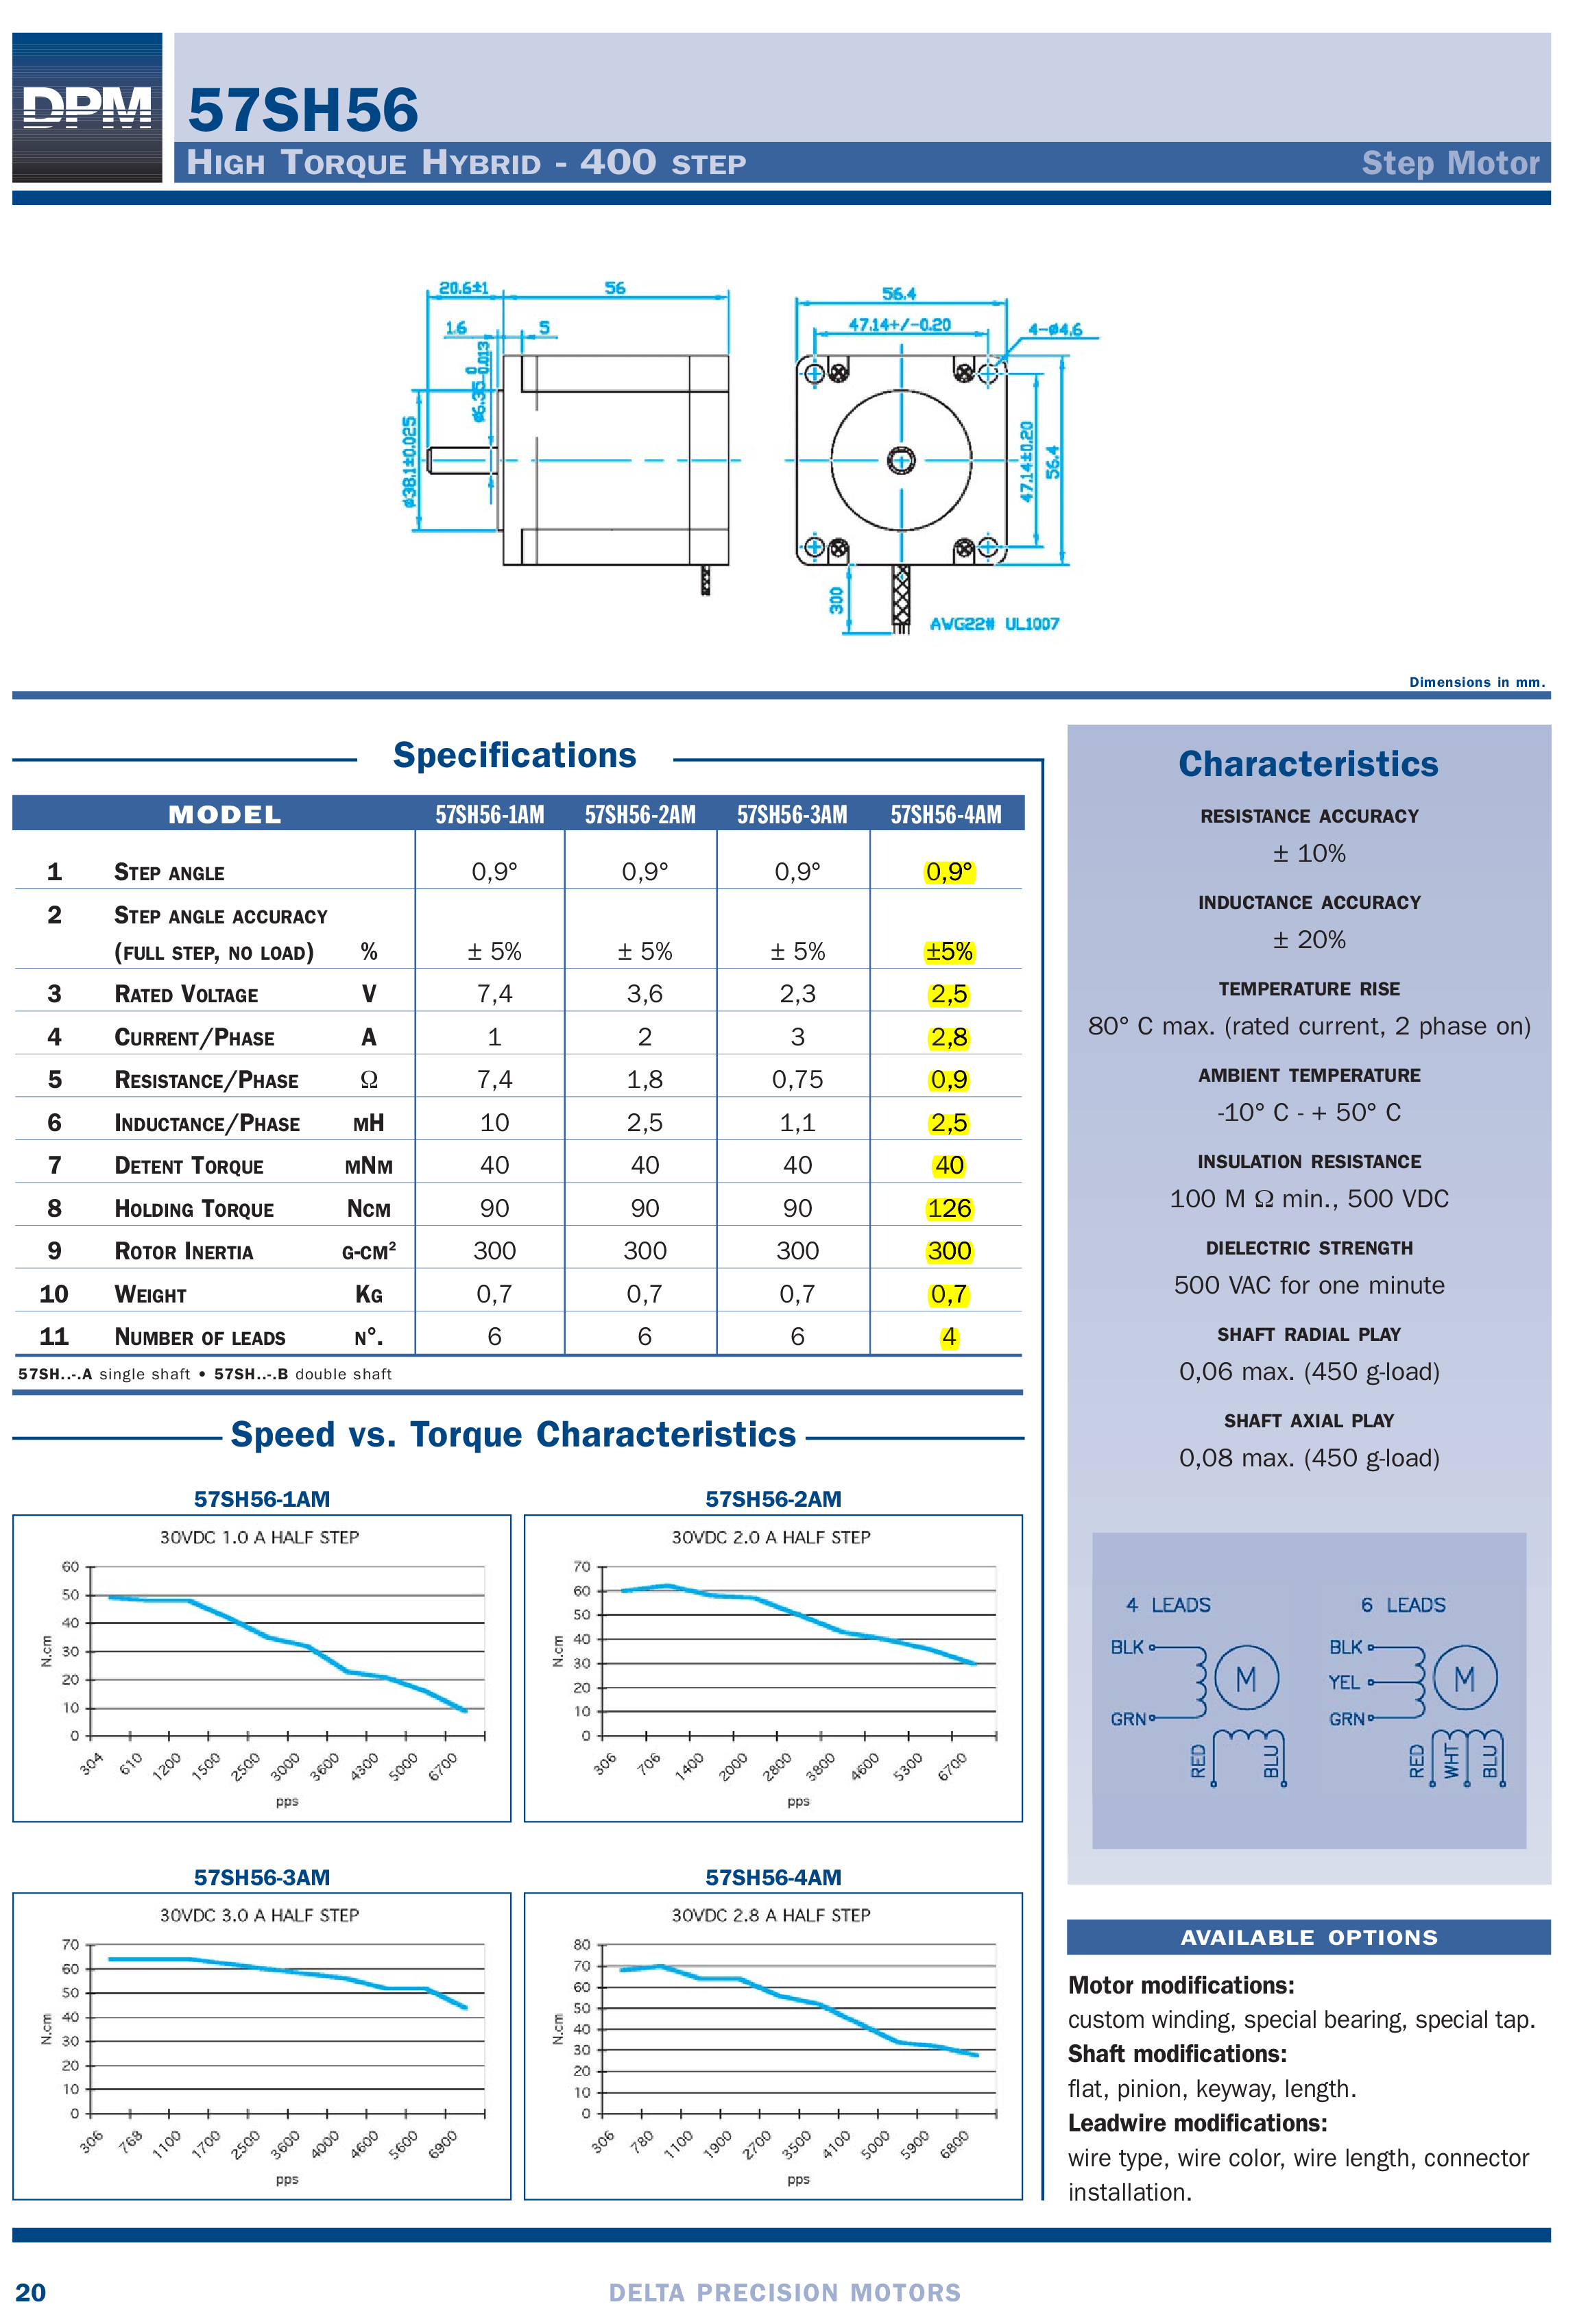
\includegraphics[width=.94\linewidth]{./files/57SH56-4AM_400_STEP} \end{center}

\hypertarget{ux3baux3b9ux3bdux3b7ux3c4ux3aeux3c1ux3b5ux3c2-filter-wheel-g11}{%
\subsection{Κινητήρες filter wheel (G11)}\label{ux3baux3b9ux3bdux3b7ux3c4ux3aeux3c1ux3b5ux3c2-filter-wheel-g11}}

\begin{center}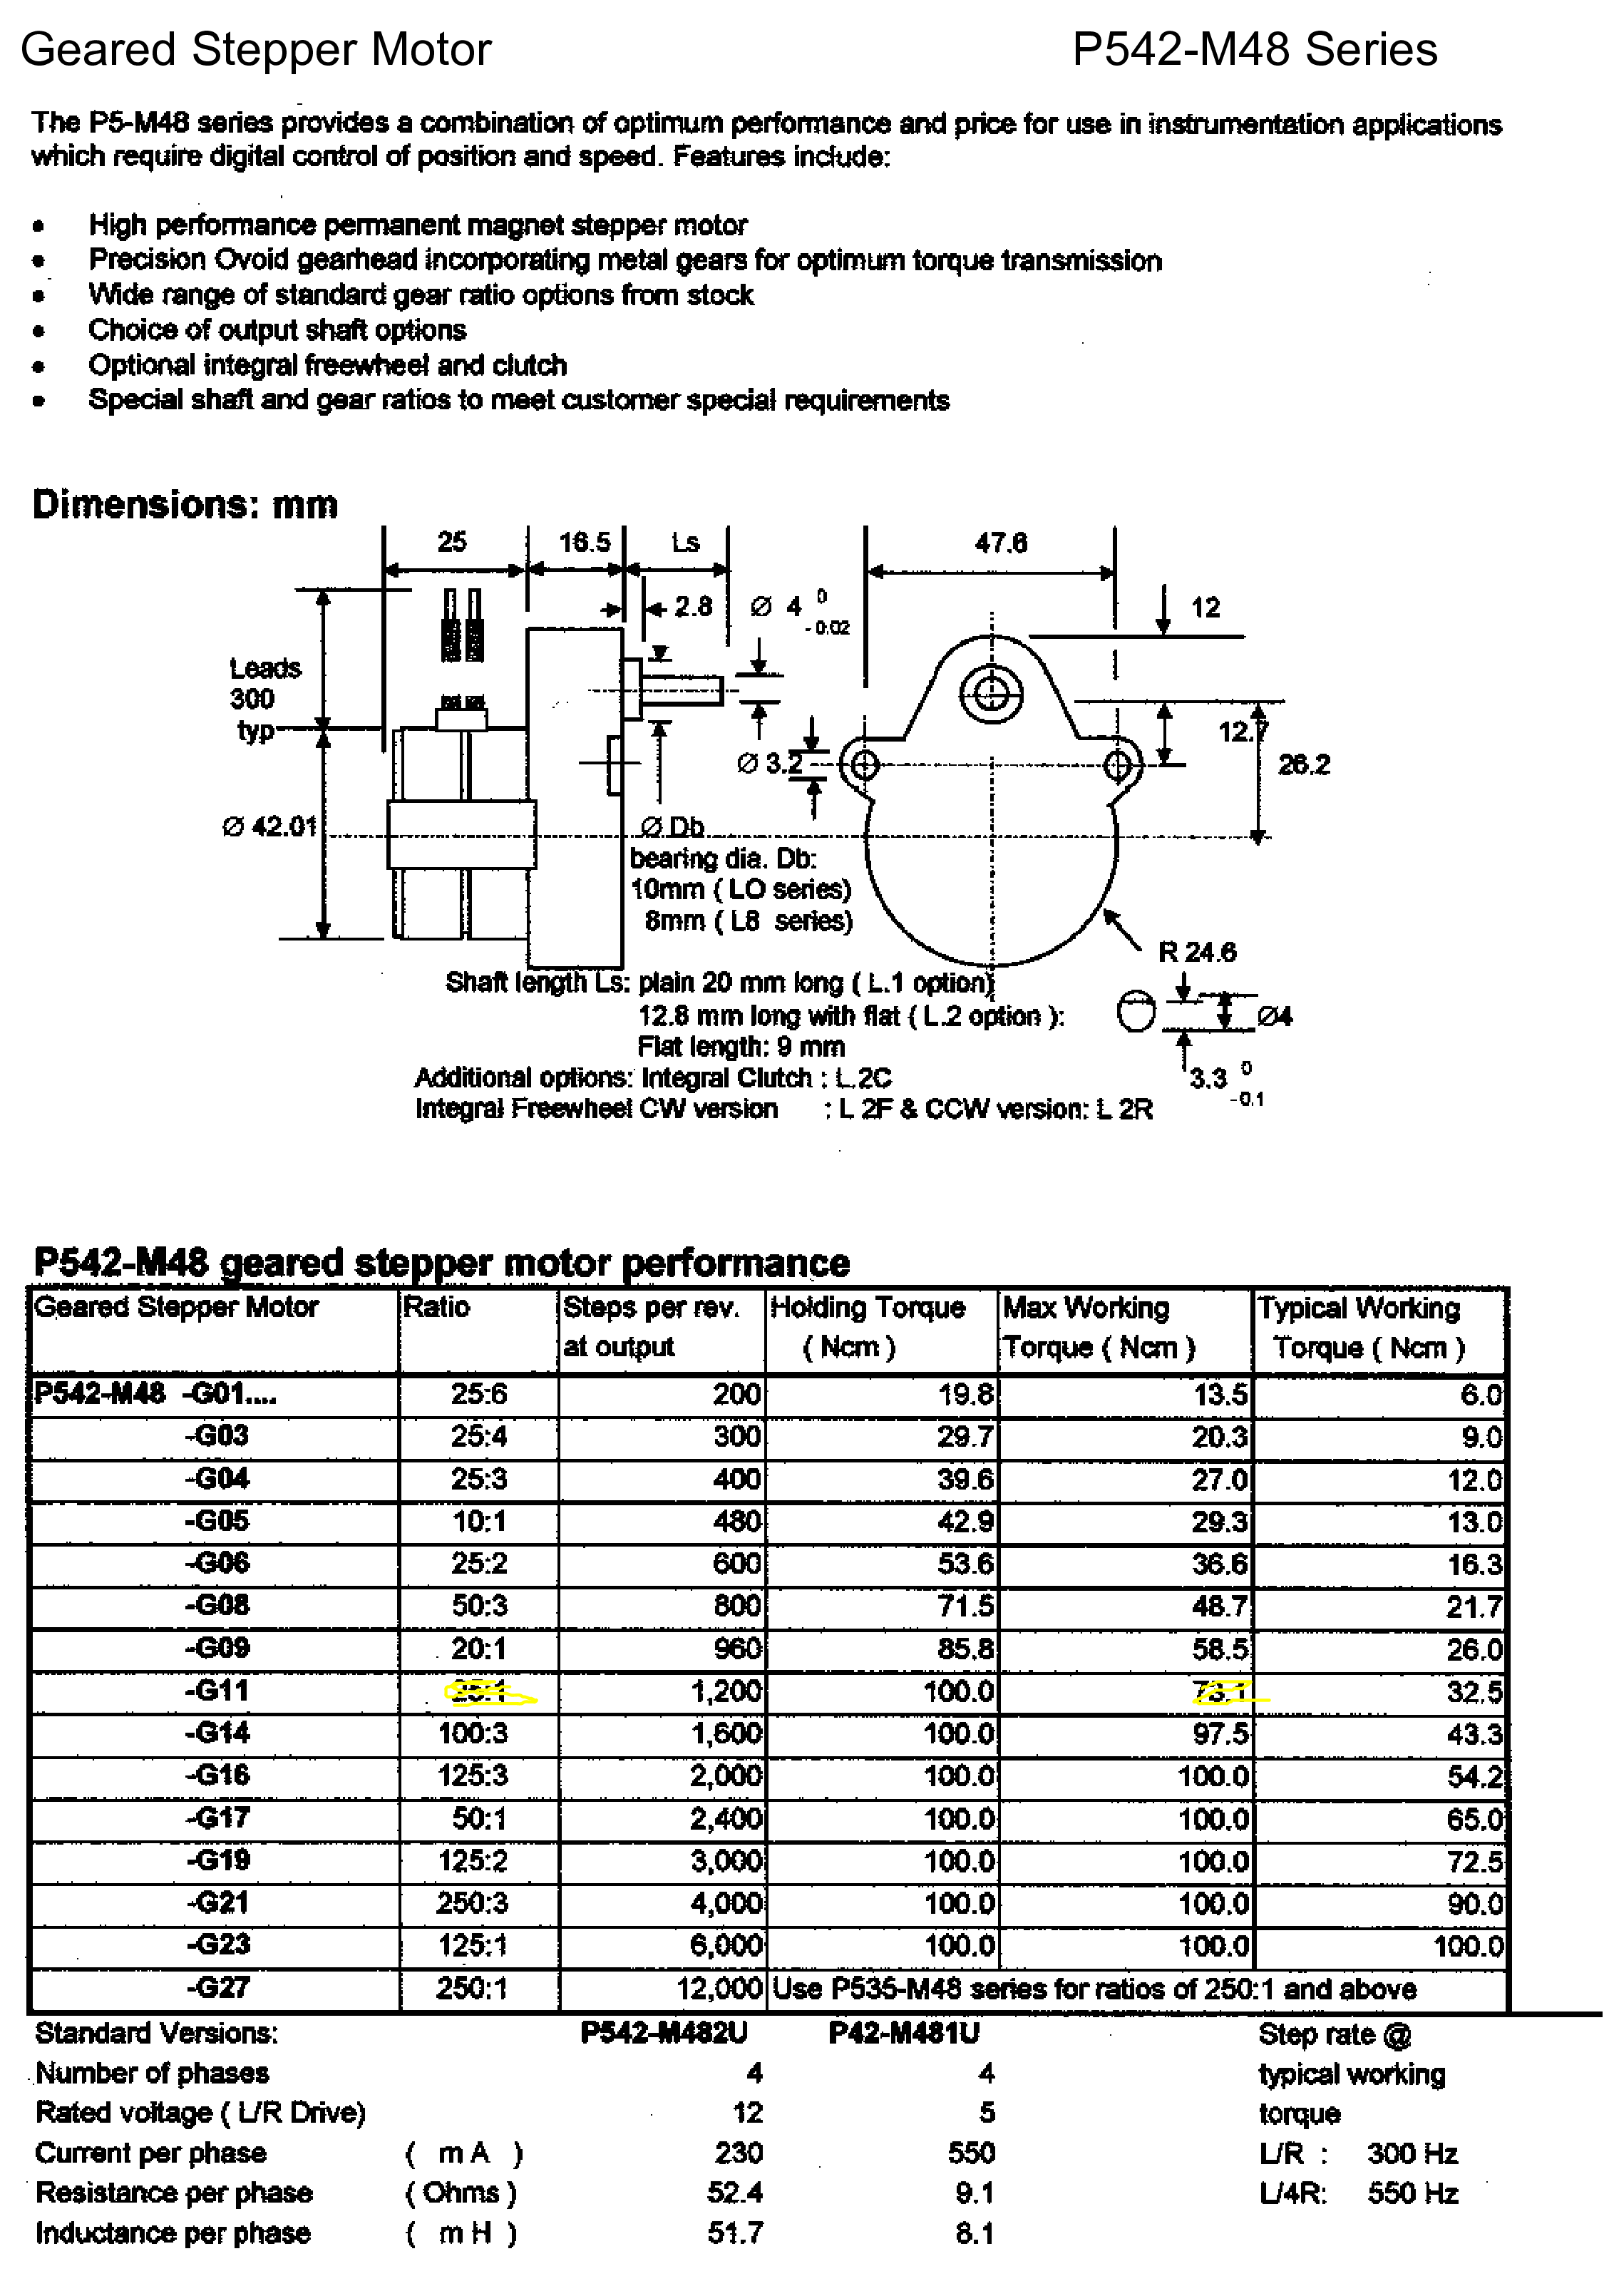
\includegraphics[width=1\linewidth]{./files/FWmotor} \end{center}

\begin{center}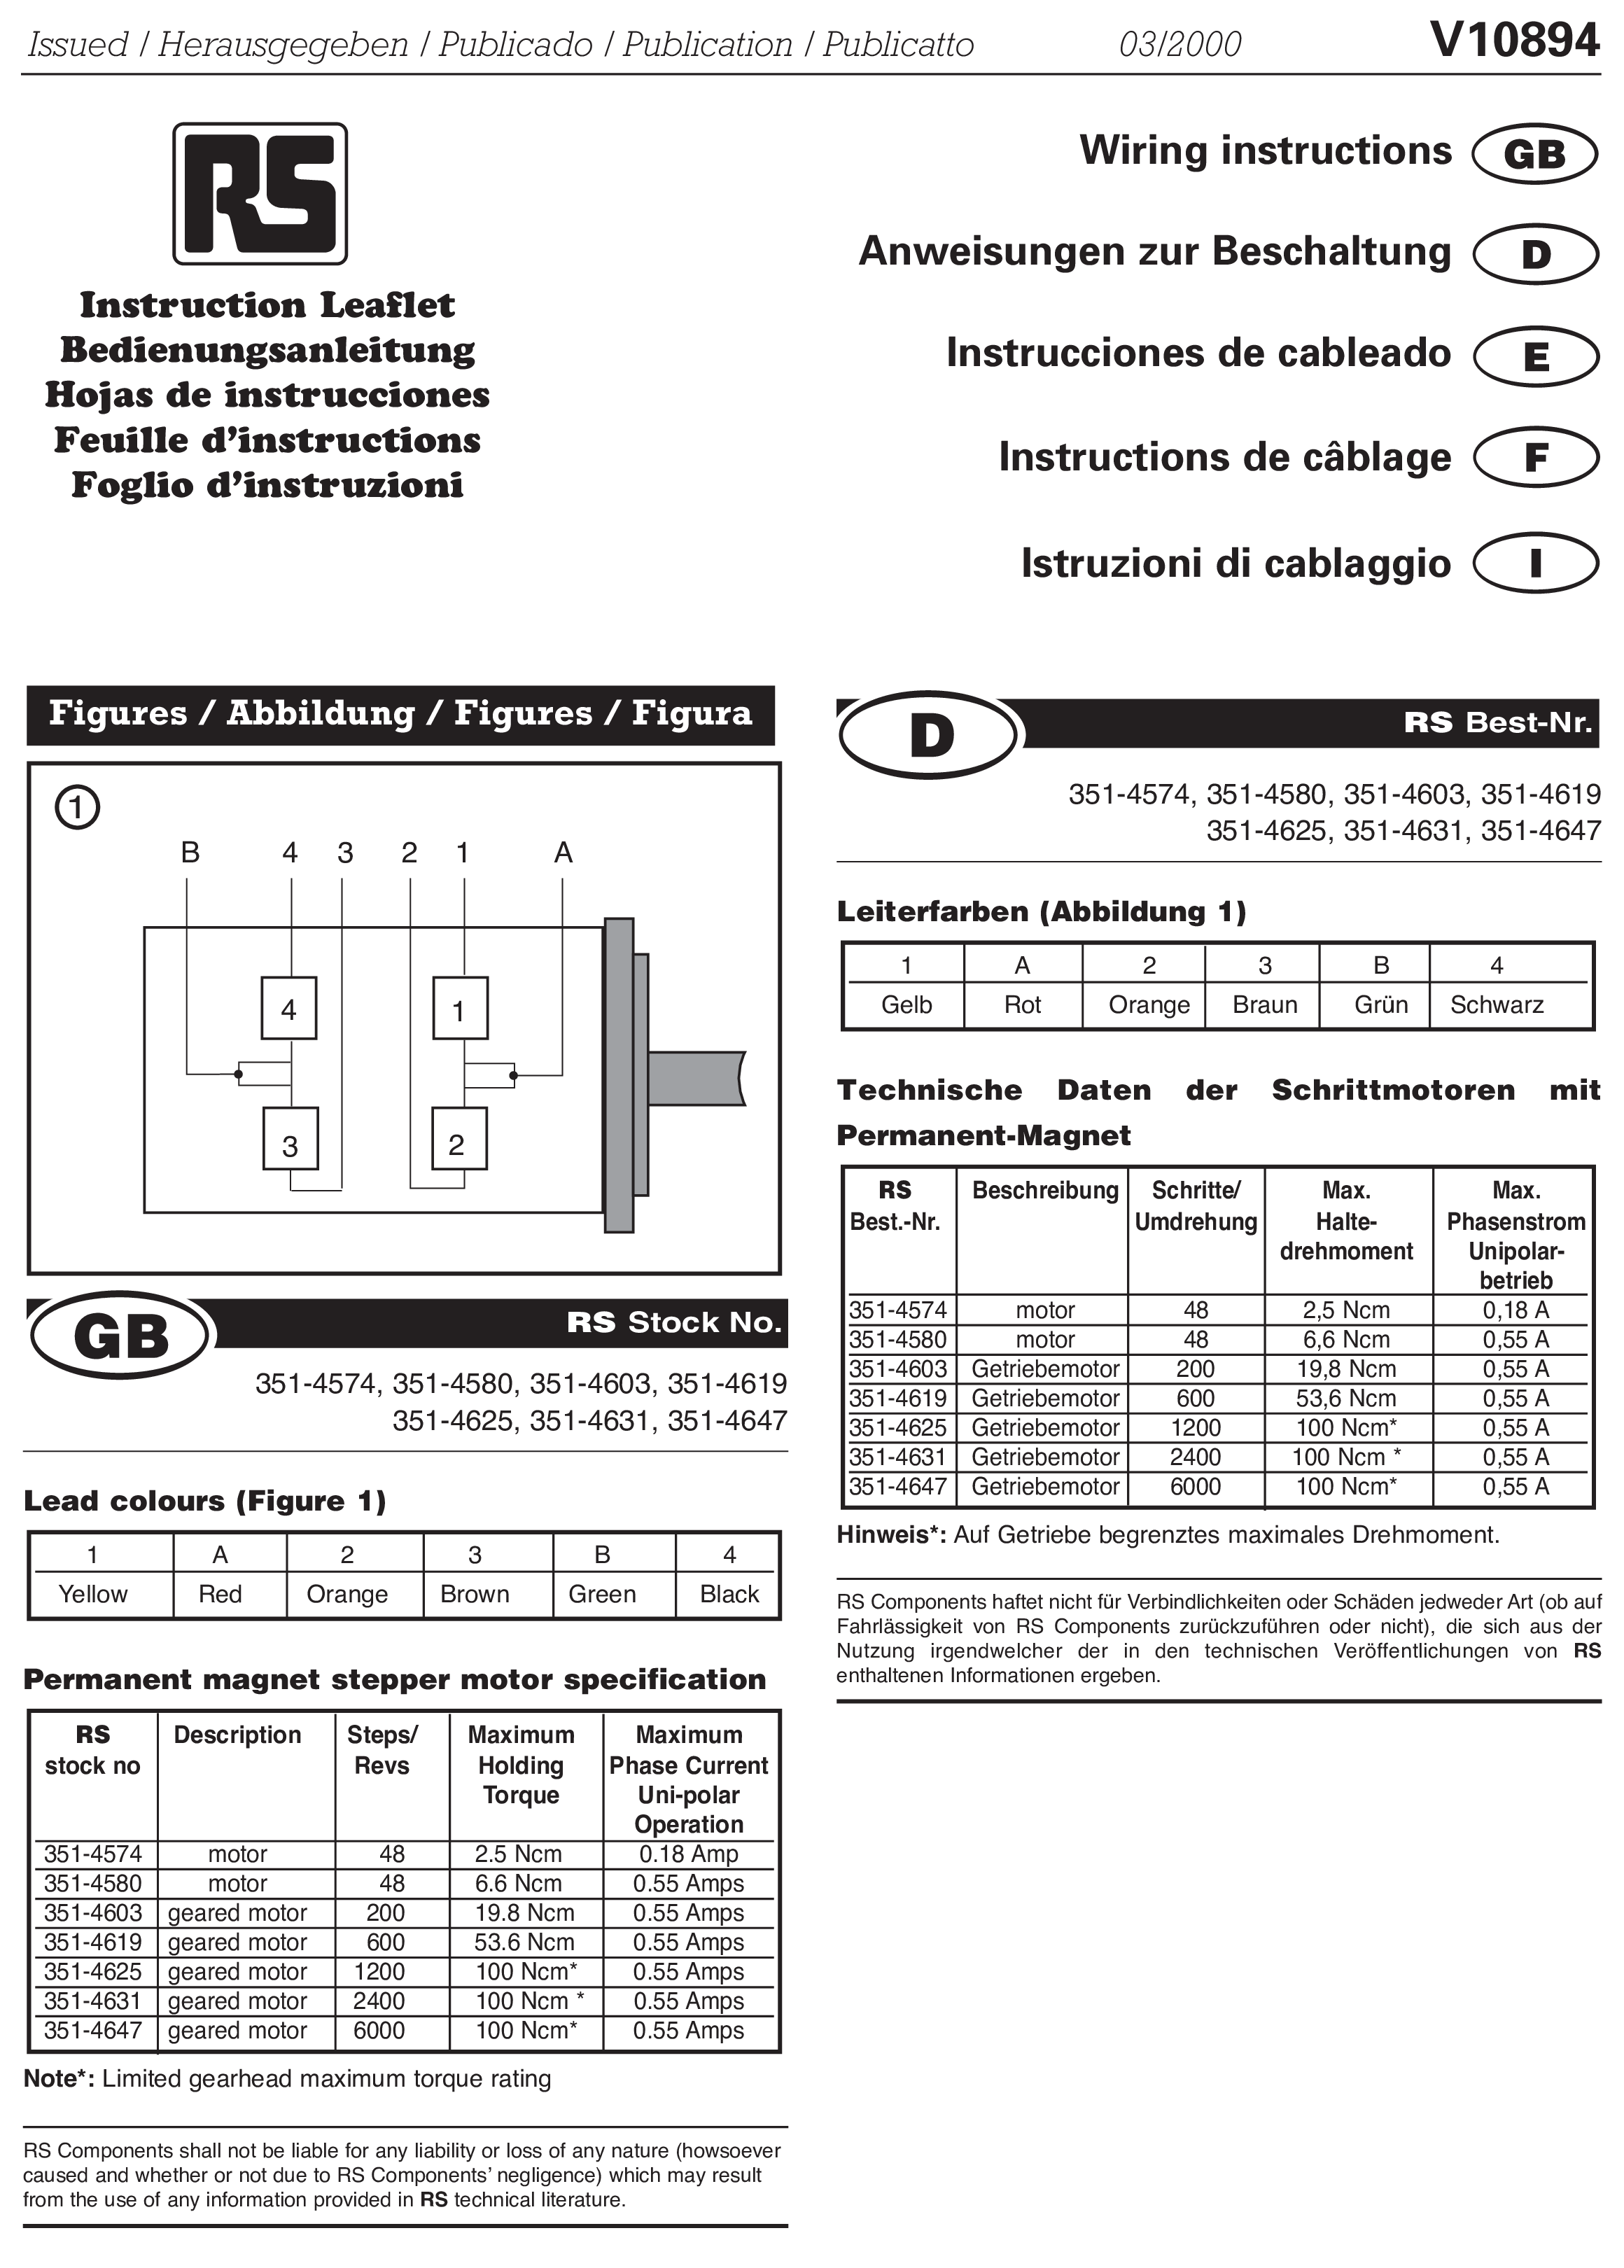
\includegraphics[width=1\linewidth]{./files/FWmotor_wiring} \end{center}

\hypertarget{ux3c4ux3c1ux3bfux3c6ux3bfux3b4ux3bfux3c3ux3afux3b1-ux3b9ux3c3ux3c7ux3cdux3bfux3c2}{%
\subsection{Τροφοδοσία ισχύος}\label{ux3c4ux3c1ux3bfux3c6ux3bfux3b4ux3bfux3c3ux3afux3b1-ux3b9ux3c3ux3c7ux3cdux3bfux3c2}}

Το τροφοδοτικό του tracker παρέχει συνεχή διαφορά δυναμικού \(19-20\ V\). Για την ώρα δεν γνωρίζουμε την δυνατότητα σε ισχύ της συσκευής ούτε φυσικά και το μέγιστο ηλεκτρικό ρεύμα που μπορεί να παρέχει.

\newpage

\hypertarget{trackerinstallation}{%
\section{Εγκατάσταση του tracker.}\label{trackerinstallation}}

Είναι αναγκαίο το επίπεδο τις συσκευής να είναι απολύτως οριζόντιο, αλλά και να διατηρείται κατά τη λειτουργία του συστήματος tracker-οργάνου. Γι' αυτό η βάση, πρέπει να είναι αρκετά σταθερή αλλά και να έχει τη δυνατότητα λεπτομερούς ρύθμισης του επιπέδου. Στη συνέχεια θα περιγράψουμε την ρύθμιση του οργάνου για την παρακολούθηση της πορείας του Ήλιου.

\begin{img}

{\centering 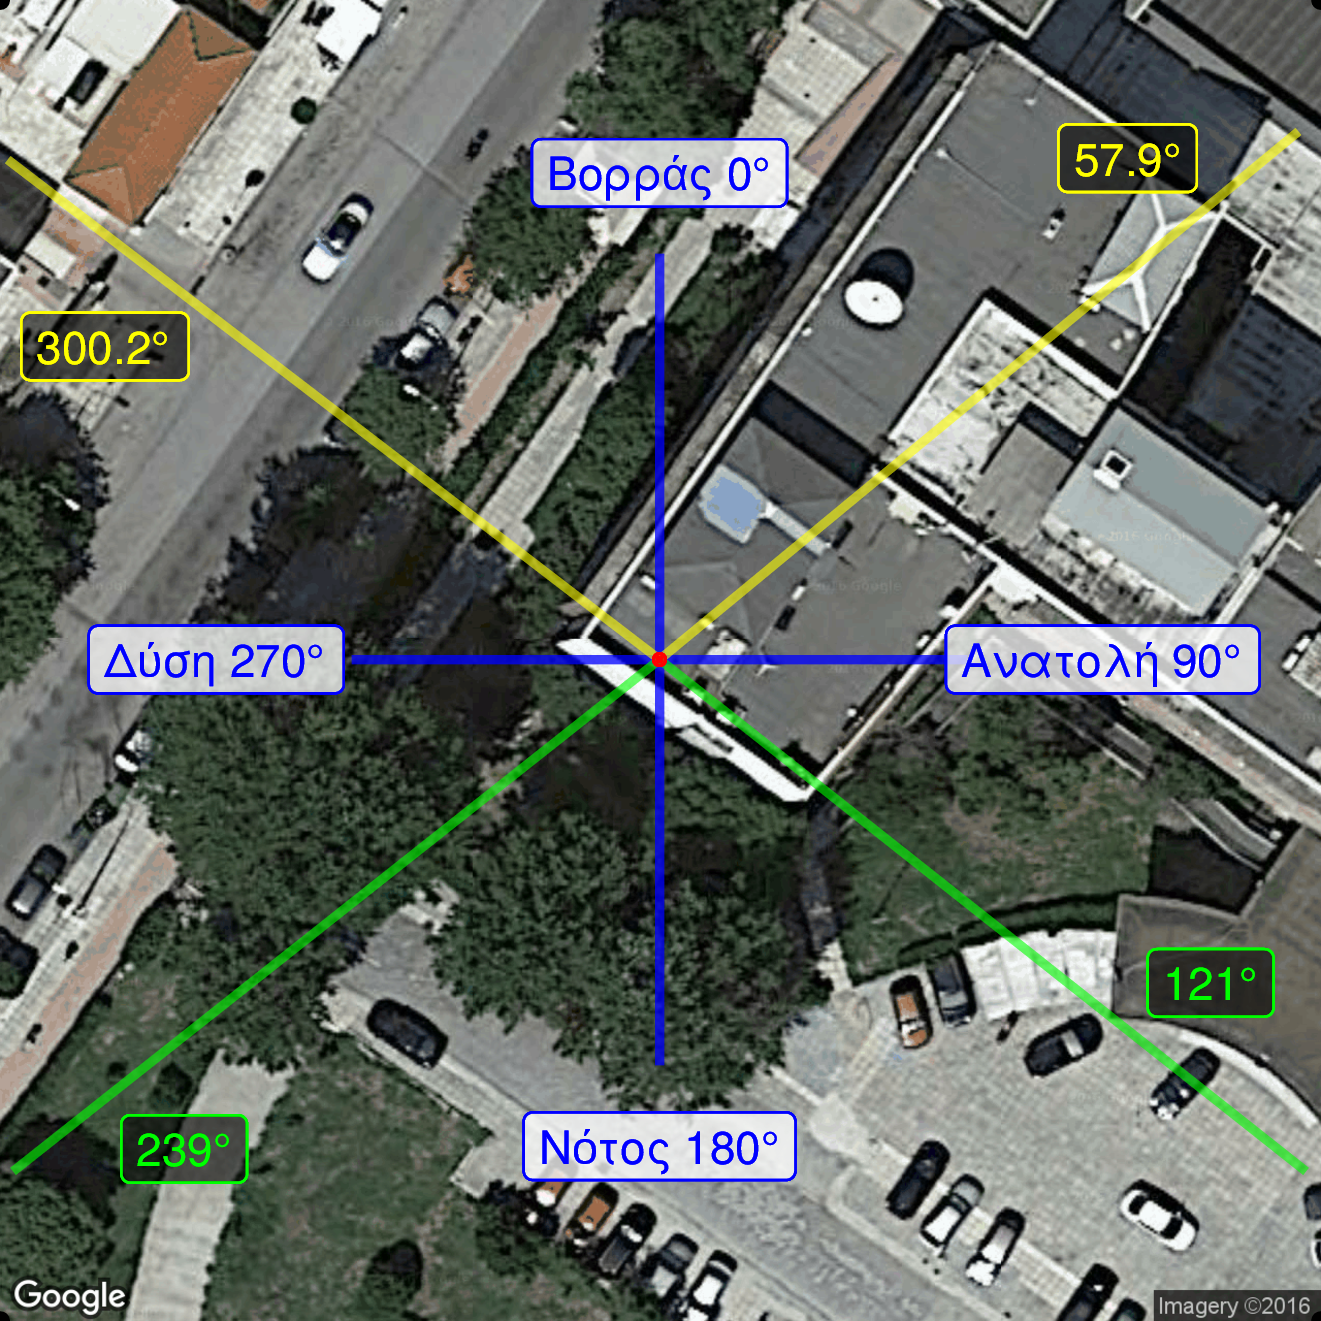
\includegraphics[width=1\linewidth]{figure/compass} 

}

\caption{Δορυφορική φωτογραφία της τοποθεσίας μετρήσεων (κόκκινο). Έχουν σχεδιαστεί οι κατευθύνσεις που αντιστοιχούν στα σημεία του ορίζοντα (μπλε), το αζιμούθιο του ήλιου κατά την ανατολή και τη δύση στις 21 Ιουλίου (κίτρινο) και αντίστοιχα στις 21 Δεκεμβρίου (πράσινο). Όλες οι γωνίες είναι μετρημένες με αρχή την κατεύθυνση του Βορρά.}\label{fig:trackercompass}
\end{img}

\hypertarget{ux3c1ux3cdux3b8ux3bcux3b9ux3c3ux3b7-ux3b1ux3b6ux3b9ux3bcux3bfux3cdux3b8ux3b9ux3bfux3c5-ux3acux3beux3bfux3bdux3b1.}{%
\subsection{Ρύθμιση αζιμούθιου άξονα.}\label{ux3c1ux3cdux3b8ux3bcux3b9ux3c3ux3b7-ux3b1ux3b6ux3b9ux3bcux3bfux3cdux3b8ux3b9ux3bfux3c5-ux3acux3beux3bfux3bdux3b1.}}

Πρώτο βήμα, είναι η ευθυγράμμιση του μηδέν του αζιμούθιου της συσκευής με τον Βορρά. Αυτό μπορεί να γίνει με άμεση ευθυγράμμιση, αν η θέση του Βορρά είναι γνωστή (Εικόνα \ref{fig:trackercompass}). Εναλλακτικά, μπορεί να γίνει όταν η συσκευή είναι ενεργή και ακολουθεί τον ήλιο. Τότε, η διόπτευση του ήλιου μπορεί να χρησιμοποιηθεί για να ευθυγραμμίσει το αζιμούθιο με τον Βορρά. Και στις δύο περιπτώσεις η συσκευή πρέπει να τοποθετηθεί στη βάση της και να μπορεί να περιστραφεί πριν σταθεροποιηθεί στην τελική της θέση. Περαιτέρω, βελτίωση της θέσης του μηδενός του αζιμουθιακού άξονα, μπορεί να γίνει προγραμματιστικά, με τις μεταβλητές του offset στο πρόγραμμα που τις ελέγχει.

\hypertarget{ux3c1ux3cdux3b8ux3bcux3b9ux3c3ux3b7-ux3b6ux3b5ux3bdux3afux3b8ux3b9ux3bfux3c5-ux3acux3beux3bfux3bdux3b1.}{%
\subsection{Ρύθμιση ζενίθιου άξονα.}\label{ux3c1ux3cdux3b8ux3bcux3b9ux3c3ux3b7-ux3b6ux3b5ux3bdux3afux3b8ux3b9ux3bfux3c5-ux3acux3beux3bfux3bdux3b1.}}

Για τον ζενίθιο άξονα, δεν θα χρειαστεί κάποια διαδικασία από τη στιγμή που η συσκευή είναι οριζοντιωμένη. Αν γνωρίζουμε τη θέση αναφοράς όπου μηδενίζει το όργανο, μπορούμε να υπολογίσουμε την θέση που ο άξονας θα βρίσκεται στο ζενίθ ή κάθετα σε αυτό (ανάλογα με τη βάση πρόσδεσης του οργάνου). Έτσι, μπορούμε να θέσουμε αυτήν την παράμετρο στο πρόγραμμα που ελέγχει τη συσκευή. Μία άλλη προσέγγιση, για να βρούμε το offset της στόχευσης, είναι η προσάρτηση του οργάνου να γίνει ενώ ο tracker ακολουθεί τον ήλιο, ώστε να ευθυγραμμιστεί με αυτόν. Αυτό προϋποθέτει ότι η στερέωση του οργάνου μπορεί να γίνει σε οποιαδήποτε γωνία σε σχέση με τον άξονα.

\hypertarget{ux3bfux3c1ux3b9ux3b6ux3bfux3bdux3c4ux3afux3c9ux3c3ux3b7-ux3c4ux3bfux3c5-ux3b7ux3bbux3b9ux3bfux3c3ux3c4ux3acux3c4ux3b7-leveling.}{%
\subsection{Οριζοντίωση του ηλιοστάτη (leveling).}\label{ux3bfux3c1ux3b9ux3b6ux3bfux3bdux3c4ux3afux3c9ux3c3ux3b7-ux3c4ux3bfux3c5-ux3b7ux3bbux3b9ux3bfux3c3ux3c4ux3acux3c4ux3b7-leveling.}}

Τέλος, έχουμε την καθετοποίηση του οργάνου, ώστε ο άξονας του αζιμούθιου να είναι κατακόρυφος στη Γη. Μετά την τοποθέτηση των οργάνων μέτρησης, αλλά και περιοδικά, η καθετότητα του άξονα πρέπει να ελέγχεται. Καθώς, αποκλίσεις μπορούν να προκαλέσουν εσφαλμένες μετρήσεις κατά τη διάρκεια της ημέρας. Η ανάγκη αυτή, μπορεί να φανεί όταν μετά από διόπτευση (sighting) του Ήλιου, ο tracker χάνει γρήγορα την ευθυγράμμισή του.

Ξεκινάμε με τον tracker χωρίς τροφοδοσία, ώστε να μπορεί να περιστραφεί ελεύθερα γύρω από τον κατακόρυφο άξονα. Για τον έλεγχο της στάθμης χρησιμοποιούμε αλφάδι φυσαλίδας (αεροστάθμη) με δυνατότης ανεξάρτητης ρύθμισης του επιπέδου του σε σχέση με το όργανο, όπως φαίνεται στην Εικόνα \ref{fig:trackerleveling}.

\begin{img}

{\centering \includegraphics[width=0.8\linewidth]{../../Aerosols/Photos/EL/20160307_Tracker_CHP1_CCD/P1110530} 

}

\caption{Οριζοντίωση του tracker. Φαίνεται ο tracker εγκατεστημένος σε ρυθμιζόμενη βάση (τρίποδο) και η αεροστάθμη (αλφάδι) με την οποία ελέγχεται η οριζοντίωση.}\label{fig:trackerleveling}
\end{img}

Θα ρυθμίσουμε κάθε σημείο ελευθερίας του επιπέδου (εδώ, κάθε πόδι της βάσης) διαδοχικά, μέχρι το επίπεδο του οργάνου να συμφωνεί με το επίπεδο αναφοράς της στάθμης. Σε όλη τη διαδικασία δεν πρέπει να αλλάξουμε τη θέση του οργάνου της στάθμης πάνω στο όργανο.

Η διαδικασία για κάθε πόδι έχει ως εξής:
Φέρνουμε τον άξονα της φυσαλίδας παράλληλο με την διεύθυνση του ποδιού. Αλλάζουμε το ύψος του και ρυθμίζουμε ξανά το όργανο στάθμης, προσπαθώντας να μοιράσουμε την μεταβολή ισόποσα μεταξύ των δύο. Περιστρέφουμε τον tracker κατά \(180^\circ\) και επαναλαμβάνουμε τη ρύθμιση και των δύο.

Το παραπάνω βήμα, το επαναλάβουμε μέχρι η στάθμη να είναι ικανοποιητικά επίπεδη. Με τον ίδιο τρόπο ρυθμίζουμε διαδοχικά και τα υπόλοιπα πόδια. Πιθανότατα, θα χρειαστεί παραπάνω από ένας κύκλος ρυθμίσεων και για το κάθε πόδι, αλλά και για τα τρία σε αλληλουχία. Το πλήθος τους, θα εξαρτηθεί από την ευαισθησία του μηχανισμού ρύθμισης, την ικανότητα του χειριστή αλλά και το επιθυμητό επίπεδο ακρίβειας.

Επαναλαμβάνουμε ότι είναι σημαντική η περιστροφή tracker μαζί με όργανο στάθμης κατά \(180^\circ\), διότι πρέπει να ληφθεί υπόψη ότι το κάλυμμα του οργάνου δεν είναι κατ' ανάγκη παράλληλο με τη βάση του (π.χ. μπορεί να έχει παραμορφωθεί).

\newpage

\appendix

\hypertarget{chp-1-quick-startup-on-radmon-computer.}{%
\section{CHP-1 Quick startup (on `radmon' computer).}\label{chp-1-quick-startup-on-radmon-computer.}}

\hypertarget{ux3c3ux3cdux3bdux3b4ux3b5ux3c3ux3b7-ux3c4ux3bfux3c5-tracker.}{%
\subsection*{Σύνδεση του tracker.}\label{ux3c3ux3cdux3bdux3b4ux3b5ux3c3ux3b7-ux3c4ux3bfux3c5-tracker.}}
\addcontentsline{toc}{subsection}{Σύνδεση του tracker.}

\vspace{-0.6\baselineskip}

Στο τροφοδοτικό του tracker συνδέονται τρία καλώδια.
Συνήθως, η σύνδεση πετυχαίνει αν τα καλώδια συνδεθούν με τη σειρά από δεξιά προς τα αριστερά ή το αντίθετο.
Η εκτέλεση του προγράμματος θα δείξει αν η επικοινωνία μπορεί να γίνει σωστά.

\vspace{-1.05\baselineskip}

\hypertarget{reset-tracker.}{%
\subsection*{Reset tracker.}\label{reset-tracker.}}
\addcontentsline{toc}{subsection}{Reset tracker.}

\vspace{-0.6\baselineskip}

Όταν ο tracker τροφοδοτείται τα ηλεκτρονικά του είναι ενεργά, μερικές φορές, αυτό αποτρέπει την επανασύνδεση.
Για να λυθεί αυτό ή πρέπει να μείνει για μερικά λεπτά χωρίς τροφοδοσία, ή να βραχυκυκλωθούν οι επαφές που τροφοδοτούν την ηλεκτρονική πλακέτα του tracker.
\textbf{ΠΡΟΣΟΧΗ: εφαρμόστε λογική και αποσυνδέστε πρώτα την τροφοδοσία ρεύματος}.
Αν το περίβλημα του tracker είναι ανοικτό, οι επαφές είναι προσβάσιμες. Εναλλακτικά, μπορούν να βραχυκυκλωθούν οι επαφές του καλωδίου με κάποιο μεταλλικό αντικείμενο και μόνο από τη μεριά του καλωδίου που συνδέεται στο τροφοδοτικό, ώστε να είστε σίγουροι για τη κατάσταση τροφοδοσίας.

\vspace{-1.05\baselineskip}

\hypertarget{ux3b5ux3baux3baux3afux3bdux3b7ux3c3ux3b7-ux3c4ux3bfux3c5-ux3c0ux3c1ux3bfux3b3ux3c1ux3acux3bcux3bcux3b1ux3c4ux3bfux3c2-ux3b5ux3bbux3adux3b3ux3c7ux3bfux3c5}{%
\subsection*{Εκκίνηση του προγράμματος ελέγχου}\label{ux3b5ux3baux3baux3afux3bdux3b7ux3c3ux3b7-ux3c4ux3bfux3c5-ux3c0ux3c1ux3bfux3b3ux3c1ux3acux3bcux3bcux3b1ux3c4ux3bfux3c2-ux3b5ux3bbux3adux3b3ux3c7ux3bfux3c5}}
\addcontentsline{toc}{subsection}{Εκκίνηση του προγράμματος ελέγχου}

\vspace{-0.6\baselineskip}

Το πρόγραμμα ελέγχου του tracker (\textbf{sun\_tracker\_main.py}) μπορεί να ξεκινήσει:

\begin{itemize}
\tightlist
\item
  Χειροκίνητα (link στην επιφάνεια εργασίας)
\item
  Μέσω του `Scheduled Tasks' (properties -\textgreater{} run)
\item
  Εκτέλεση από command line (cmd.exe):
\end{itemize}

\begin{Shaded}
\begin{Highlighting}[]
\ExtensionTok{c:\textbackslash{}\textgreater{}}\OperatorTok{\textless{}}\NormalTok{python path}\OperatorTok{\textgreater{}}\DataTypeTok{\textbackslash{}p}\NormalTok{ython.exe }\OperatorTok{\textless{}}\NormalTok{script path}\OperatorTok{\textgreater{}}\DataTypeTok{\textbackslash{}s}\NormalTok{un\_tracker\_main.py}
\end{Highlighting}
\end{Shaded}

\vspace{-1.05\baselineskip}

\hypertarget{ux3b4ux3b9ux3ccux3c0ux3c4ux3b5ux3c5ux3c3ux3b7-sighting}{%
\subsection*{Διόπτευση (sighting)}\label{ux3b4ux3b9ux3ccux3c0ux3c4ux3b5ux3c5ux3c3ux3b7-sighting}}
\addcontentsline{toc}{subsection}{Διόπτευση (sighting)}

\vspace{-0.6\baselineskip}

Το sighting του Ήλιου μπορεί να γίνει με το πρόγραμμα \textbf{tracker\_sighting\_no\_ui\_tcp-port.py} (υπάρχει link στην επιφάνεια εργασίας).
Το πρόγραμμα εμφανίζει τις δυνατές επιλογές στην οθόνη και περιμένει είσοδο από το πληκτρολόγιο.
Οι ρυθμίσεις επιδρούν άμεσα στη θέση του tracker (το πρόγραμμα \textbf{sun\_tracker\_main.py} πρέπει να εκτελείται και ο tracker πρέπει να έχει αρχίσει την κανονική λειτουργία).
Ανάδραση (feedback) των ρυθμίσεων μπορούμε να έχουμε παρακολουθώντας το terminal που τρέχει το \textbf{sun\_tracker\_main.py}. \textbf{ΠΡΟΣΟΧΗ.} Οι ρυθμίσεις πρέπει να σωθούν (\texttt{\textquotesingle{}s\textquotesingle{}}) για να αποθηκευτούν στον δίσκο και να διατηρηθούν στην επόμενη εκτέλεση (ημέρα).

\textbf{Σημείωση:} Είναι βολικό το sighting να γίνεται με κάποιο smart phone μέσω remote desktop (`rdp').
Έτσι, μπορεί να υπάρχει άμεση επίβλεψη της κίνησης του tracker και των διορθώσεων και διευκολύνεται ο συγχρονισμός της κίνησης του tracker με τη θέση του ήλιου.

\vspace{-1.05\baselineskip}

\hypertarget{ux3c3ux3cdux3bdux3b4ux3b5ux3c3ux3b7-ux3c0ux3bfux3bbux3c5ux3bcux3adux3c4ux3c1ux3bfux3c5-protek-506}{%
\subsection*{Σύνδεση πολυμέτρου `Protek 506'}\label{ux3c3ux3cdux3bdux3b4ux3b5ux3c3ux3b7-ux3c0ux3bfux3bbux3c5ux3bcux3adux3c4ux3c1ux3bfux3c5-protek-506}}
\addcontentsline{toc}{subsection}{Σύνδεση πολυμέτρου `Protek 506'}

\vspace{-0.6\baselineskip}

Το πολύμετρο μετράει την αντίσταση του pt100 ή του θερμίστορ (χρωματισμός καλωδίων στο manual του CHP) και η μέτρηση διαβάζεται μέσω `RS-232'.
Στο πολύμετρο πρέπει να είναι ενεργές οι επιλογές `\emph{KEEP ON}' και `\emph{RS232}'. Αυτό γίνεται με τα πλήκτρα `menu' και `enter' για κάθε μία από τις ρυθμίσεις.

\vspace{-1.05\baselineskip}

\hypertarget{ux3b5ux3baux3baux3afux3bdux3b7ux3c3ux3b7-ux3c0ux3c1ux3bfux3b3ux3c1ux3acux3bcux3bcux3b1ux3c4ux3bfux3c2-ux3c0ux3bfux3bbux3c5ux3bcux3adux3c4ux3c1ux3bfux3c5}{%
\subsection*{Εκκίνηση προγράμματος πολυμέτρου}\label{ux3b5ux3baux3baux3afux3bdux3b7ux3c3ux3b7-ux3c0ux3c1ux3bfux3b3ux3c1ux3acux3bcux3bcux3b1ux3c4ux3bfux3c2-ux3c0ux3bfux3bbux3c5ux3bcux3adux3c4ux3c1ux3bfux3c5}}
\addcontentsline{toc}{subsection}{Εκκίνηση προγράμματος πολυμέτρου}

\vspace{-0.6\baselineskip}

Το πρόγραμμα (\textbf{protek506\_measurments.py}) παίρνει μετρήσεις της αντίστασης - θερμοκρασίας του CHP1 και μπορεί να εκτελεστεί με όμοιο τρόπο με το πρόγραμμα του tracker.
Καθώς το πρόγραμμα παίρνει μετρήσεις, στη οθόνη του πολυμέτρου πρέπει να αναβοσβήνουν εναλλάξ οι ενδείξεις `\emph{RX}' και `\emph{TX}'.
Αν αυτό δεν γίνεται τότε η επικοινωνία έχει κολλήσει και το πολύμετρο πρέπει να κλείσει, να ξανανοίξει και να ρυθμιστεί (όπως παραπάνω).

\vspace{-1.05\baselineskip}

\hypertarget{ux3c3ux3b5-ux3c0ux3b5ux3c1ux3afux3c0ux3c4ux3c9ux3c3ux3b7-ux3b4ux3b9ux3b1ux3baux3bfux3c0ux3aeux3c2-ux3c1ux3b5ux3cdux3bcux3b1ux3c4ux3bfux3c2.}{%
\subsection*{Σε περίπτωση διακοπής ρεύματος.}\label{ux3c3ux3b5-ux3c0ux3b5ux3c1ux3afux3c0ux3c4ux3c9ux3c3ux3b7-ux3b4ux3b9ux3b1ux3baux3bfux3c0ux3aeux3c2-ux3c1ux3b5ux3cdux3bcux3b1ux3c4ux3bfux3c2.}}
\addcontentsline{toc}{subsection}{Σε περίπτωση διακοπής ρεύματος.}

\vspace{-0.6\baselineskip}

Έχει παρατηρηθεί ότι ο tracker μπορεί να ξεκινήσει κανονικά όταν επανέλθει η τροφοδοσία και ξεκινήσει ο υπολογιστής. Αλλά αυτό δεν γίνεται πάντα.

\vspace{-1\baselineskip}

\hypertarget{scheduled-script-description}{%
\subsection*{Scheduled script description}\label{scheduled-script-description}}
\addcontentsline{toc}{subsection}{Scheduled script description}

\vspace{-0.7\baselineskip}

Τα παρακάτω script εκτελούνται συνεχώς από το `Task Scheduler' και σχετίζονται με τη καθημερινή λειτουργία του tracker και του CPH1, και είναι:

\begin{itemize}
\tightlist
\item
  \textbf{sun\_tracker\_main.py} (απαραίτητο, ελέγχει την κίνηση του tracker)
\item
  \textbf{protek506\_measurments.py} (σημαντικό, μετράει την θερμοκρασία του CPH1)
\item
  \textbf{data\_pub\_win.py} (βοηθητικό, εκπέμπει δεδομένα λειτουργίας του tracker)
\end{itemize}

\textbf{Σημείωση:} Σε περίπτωση που κάποιο από αυτά ήδη εκτελείται δεν θα ξανατρέξει, διότι υπάρχει εσωτερικός έλεγχος στον κώδικα του κάθε προγράμματος.

\textbf{Σημείωση:} Πρέπει να είναι είναι ενεργή η επιλογή: \texttt{"Disable\ error\ reporting"} ώστε να μην κολλάει ο tracker περιμένοντας τον διάλογο του ``Error reporting'' όταν crashάρει. Πιθανόν και η επιλογή \texttt{"But\ notify\ me\ when\ critical\ error\ occurs"} (υπό δοκιμή για την ώρα). Για \emph{Windows XP: Control Panel \textgreater{} System \textgreater{} Advanced \textgreater{} Error reporting}.

\hypertarget{tracker-microcontroler-source-code}{%
\section{Tracker microcontroler source code}\label{tracker-microcontroler-source-code}}

\tiny

\begin{verbatim}
#include    <htc.h>
__CONFIG(FOSC_INTOSC&WDTE_ON&PWRTE_OFF&MCLRE_OFF&CP_ON&CPD_ON&BOREN_ON&CLKOUTEN_OFF&IESO_OFF&FCMEN_OFF);
__CONFIG(WRT_ALL&PLLEN_OFF&STVREN_ON&LVP_OFF);//&BORV_25

#pragma warning disable 340

#define _XTAL_FREQ 16000000

#define BIT0        0b00000001
#define BIT1        0b00000010
#define BIT2        0b00000100 
#define BIT3        0b00001000
#define BIT4        0b00010000
#define BIT5        0b00100000
#define BIT6        0b01000000
#define BIT7        0b10000000
#define BIT0_       0b11111110
#define BIT1_       0b11111101
#define BIT2_       0b11111011
#define BIT3_       0b11110111
#define BIT4_       0b11101111
#define BIT5_       0b11011111
#define BIT6_       0b10111111
#define BIT7_       0b01111111


#define PIN_A_A1_L              LATE1
#define PIN_A_A1_H              LATE2
#define PIN_A_A2_L              LATE0
#define PIN_A_A2_H              LATA5
#define PIN_A_B1_L              LATA1
#define PIN_A_B1_H              LATA4
#define PIN_A_B2_L              LATA2
#define PIN_A_B2_H              LATA3


#define PIN_Z_A1_L              LATD0
#define PIN_Z_A1_H              LATD1
#define PIN_Z_A2_L              LATC3
#define PIN_Z_A2_H              LATC2
#define PIN_Z_B1_L              LATC0
#define PIN_Z_B1_H              LATC1
#define PIN_Z_B2_L              LATA6
#define PIN_Z_B2_H              LATA7

#define PIN_F_A1_L              LATD3
#define PIN_F_A1_H              LATD2
#define PIN_F_A2_L              LATC4
#define PIN_F_A2_H              LATC5
#define PIN_F_B1_L              LATD5
#define PIN_F_B1_H              LATD4
#define PIN_F_B2_L              LATD6
#define PIN_F_B2_H              LATD7


#define PIN_A_OPTO              RB2
#define PIN_Z_OPTO              RB3
#define PIN_F_OPTO              RB4



#define OA_Mem                  10
#define OZ_Mem                  20
#define OF_Mem                  30

#define SpeedA_Mem              40
#define SpeedZ_Mem              41
#define SpeedF_Mem              42

#define DA_Mem                  50
#define DZ_Mem                  60
#define DF_Mem                  70

#define AZ_Mem                  90



const unsigned char StepMotorMatrix[5]={  // A1L A1H A2L A2H B1L B1H B2L B2H  
0b00000000,// OFF 
0b10010000,//
0b00001001,//
0b01100000,//
0b00000110 //
};



unsigned char TX_out;
unsigned char RX_in;


unsigned char Mem_Data;
unsigned char Mem_Address;

unsigned int  TxFSM;
unsigned char TxChar;
unsigned int  TxStringCounter;

unsigned int  RxFSM;
unsigned char RxChar;
unsigned int  RxCounter;

/*
unsigned int  ADC_tempResult;
unsigned char Counter_ADC_Sum;
unsigned int  I1_Sum;
unsigned int  I2_Sum;
unsigned int  I3_Sum;
unsigned int  I4_Sum;
unsigned int  I5_Sum;
unsigned int  I1_Sum_temp;
unsigned int  I2_Sum_temp;
unsigned int  I3_Sum_temp;
unsigned int  I4_Sum_temp;
unsigned int  I5_Sum_temp;
*/


unsigned char Counter100usec;
unsigned char Counter1msec;
unsigned char Counter10msec;
unsigned char Counter100msec;
unsigned char Counter1sec=50;

unsigned int  ITD_Input;
unsigned char ITD_Output[5];

unsigned char ADCFSM=0;



unsigned int  Timer_Init=20;


unsigned char MainFSM=0;
unsigned int  MainTimer=0;


unsigned char ReceivedByte;
unsigned char ReceiveFIFO[20];
unsigned char ReceiveValid;
unsigned char ReceiveCommand;
unsigned char ReceivedBytesCounter=0;

unsigned char TX_Mirror_Matrix[10];
unsigned int  TX_Mirror_Counter=0;

unsigned char TX_Matrix[81];
unsigned int  TX_Counter;
unsigned int  TX_Counter_Max;
unsigned char SendFlag;

unsigned char TXFSM;

unsigned char StepMotorStateA=0;
unsigned char StepMotorStateZ=0;
unsigned char StepMotorStateF=0;

unsigned int  AZ=5000;
unsigned int  ZE=5000;
unsigned int  FR=5000;

unsigned int  OA=0;
unsigned int  OZ=0;
unsigned int  OF=0;

unsigned int  Init_DA=0;
unsigned int  Init_DZ=0;
unsigned int  Init_DF=0;

unsigned int  AZtarget=100;
unsigned int  ZEtarget=100;
unsigned int  FRtarget=100;

unsigned int  AZterminal=100;
unsigned int  ZEterminal=100;
unsigned int  FRterminal=100;


unsigned int  AZtarget_temp=100;
unsigned int  ZEtarget_temp=100;
unsigned int  FRtarget_temp=100;

unsigned char SpeedA=10;
unsigned char SpeedZ=10;
unsigned char SpeedF=10;

unsigned char SpeedAnow=1;
unsigned char SpeedZnow=1;
unsigned char SpeedFnow=1;

unsigned char SpeedAtarget=1;
unsigned char SpeedZtarget=1;
unsigned char SpeedFtarget=1;

unsigned char SpeedAcalc=0;
unsigned char SpeedZcalc=0;
unsigned char SpeedFcalc=0;

unsigned int  Counter_Speed_A=0;
unsigned int  Counter_Speed_Z=0;
unsigned int  Counter_Speed_F=0;

unsigned int  ReceiveNumber=0;

unsigned int  AZ_Memory=0;

unsigned int  FSM=0;

unsigned int  FSM_A=0;
unsigned int  FSM_Z=0;
unsigned int  FSM_F=0;

unsigned int  Timer_FSM_A=0;
unsigned int  Timer_FSM_Z=0;
unsigned int  Timer_FSM_F=0;



unsigned int  A_OPTO_Shift=0b0101010101010101;
unsigned int  Z_OPTO_Shift=0b0101010101010101;
unsigned int  F_OPTO_Shift=0b0101010101010101;


unsigned int  tempint;
unsigned char tempB;




bit FLAG1msec=0;

bit Moving=0;
bit OKpending=0;

bit AZsync=0;
bit ZEsync=0;
bit FRsync=0;

bit SendAll=0;

bit SendAZ=0;
bit SendZE=0;
bit SendFR=0;

bit SendOA=0;
bit SendOZ=0;
bit SendOF=0;

bit SendDA=0;
bit SendDZ=0;
bit SendDF=0;

bit SendSA=0;
bit SendSZ=0;
bit SendSF=0;

bit SendTA=0;
bit SendTZ=0;
bit SendTF=0;

bit SendOK=0;
bit SendLF=0;

bit SendDebugOff=0;
bit SendDebugOn=0;

bit Debug=0;

bit GoToTargetA=0;
bit GoToTargetZ=0;
bit GoToTargetF=0;
bit GoToTargetAll=0;

bit TargetReachedA=0;
bit TargetReachedZ=0;
bit TargetReachedF=0;
bit TargetReachedAll=0;

bit GoToTerminalA=0;
bit GoToTerminalZ=0;
bit GoToTerminalF=0;
bit GoToTerminalAll=0;

bit TerminalReachedA=0;
bit TerminalReachedZ=0;
bit TerminalReachedF=0;
bit TerminalReachedAll=0;

bit StopA=0;
bit StopZ=0;
bit StopF=0;
bit StopAll=0;

bit CounterApulse=0;
bit CounterZpulse=0;
bit CounterFpulse=0;

bit PositionValid_A=0;
bit PositionValid_Z=0;
bit PositionValid_F=0;

bit A_OPTO=0;
bit Z_OPTO=0;
bit F_OPTO=0;

void SPI(void);
void MemRead(void);
void MemWrite(void);
void ReadParameters(void);
void WriteParameters(void);
void SMS_Number_Server(void);
void SMS_Number_Mobile(void);
void ReadUPSfromFlash(void);
void SaveUPStoFlash(void);
void ReadLSfromFlash(void);
void SaveLStoFlash(void);

void SCI_Receive(void);

void ReceiveByteRoutine(void);
void TX_Routine(void);

void TX_Mirror(unsigned char TXM_byte);


void My_EE_Write(unsigned char My_EE_Adr,unsigned char My_EE_Data);
unsigned char My_EE_Read(unsigned char My_EE_Adr);
void IntToDec(void);
void ReadKeys(void);
void ADC_Routine(void);

void SetStepMotorStates(void);

void StepUpA(void);
void StepDownA(void);
void StepUpZ(void);
void StepDownZ(void);
void StepUpF(void);
void StepDownF(void);

void MoveToTargetA(void);
void MoveToTargetZ(void);
void MoveToTargetF(void);

void DummyMoving(void);

void FSM_A_Routine(void);
void FSM_Z_Routine(void);
void FSM_F_Routine(void);

void ReadOPTO(void);

main()
{
unsigned char i;

CLRWDT();

IRCF3=1;
IRCF2=1;
IRCF1=1;
IRCF0=1;


PORTA =0b00000000;
TRISA =0b00000001;
ANSELA=0b00000000;

PORTB =0b00000000;
TRISB =0b11111100;
ANSELB=0b00100000;
WPUB  =0b11011100;

PORTC =0b00000000;
TRISC =0b11000000; 

PORTD =0b00000000;
TRISD =0b00000000;
ANSELD=0b00000000;

PORTE =0b00000000;
TRISE =0b00001000;
ANSELE=0b00000000;
WPUE  =0b00001000;

nWPUEN=0;

GIE = 0;
//------------------------------------------------


//------------------------------------------------
FVRCON=0b10000011; // 4.096 V
ADCON1=0b10100011;
//------------------------------------------------

//------------------------------------------------
_delay(10000);

AZ=(My_EE_Read(AZ_Mem)<<8)+My_EE_Read(AZ_Mem+1);
if (AZ>9999) {AZ=100;}
AZtarget=AZ;

OA=(My_EE_Read(OA_Mem)<<8)+My_EE_Read(OA_Mem+1);
if (OA>9999) {OA=0;}
OZ=(My_EE_Read(OZ_Mem)<<8)+My_EE_Read(OZ_Mem+1);
if (OZ>9999) {OZ=0;}
OF=(My_EE_Read(OF_Mem)<<8)+My_EE_Read(OF_Mem+1);
if (OF>9999) {OF=0;}

Init_DA=(My_EE_Read(DA_Mem)<<8)+My_EE_Read(DA_Mem+1);
if (Init_DA>9999) {Init_DA=5000;}
Init_DZ=(My_EE_Read(DZ_Mem)<<8)+My_EE_Read(DZ_Mem+1);
if (Init_DZ>9999) {Init_DZ=5000;}
Init_DF=(My_EE_Read(DF_Mem)<<8)+My_EE_Read(DF_Mem+1);
if (Init_DF>9999) {Init_DF=5000;}


SpeedA=My_EE_Read(SpeedA_Mem);
if (SpeedA>99) {SpeedA=80;}
SpeedZ=My_EE_Read(SpeedZ_Mem);
if (SpeedZ>99) {SpeedZ=80;}
SpeedF=My_EE_Read(SpeedF_Mem);
if (SpeedF>99) {SpeedF=80;}


//------------------------------------------------
TxFSM=0;
RxFSM=0;


//-----------------------------------------------------------------------------------------
//-----------------------------------------------------------------------------------------
//-----------------------------------------------------------------------------------------
//-----------------------------------------------------------------------------------------
//-----------------------------------------------------------------------------------------
//-----------------------------------------------------------------------------------------

//-----------------------------------------------------------------------------------------
//-----------------------------------------------------------------------------------------
//-----------------------------------------------------------------------------------------
//-----------------------------------------------------------------------------------------
//-----------------------------------------------------------------------------------------
//-----------------------------------------------------------------------------------------


//------------------------------------------------
SPBRG=207;//4800
BAUDCON=0b00000000;
TXSTA=0b00000100;
RCSTA=0b00000000;
SPEN=1;
TXEN=1;
CREN=1;
tempB=RCSTA;
tempB=RCREG;
//------------------------------------------------

//------------------------------------------------
PSA=0;
PS2=0;
PS1=0;
PS0=0;
T0CS=0;
TMR0IE=1;
//------------------------------------------------

GIE = 1;            // enable global interrupts



while (1)
    {
    CLRWDT();


    if (FLAG1msec) // ---------------1msec-------------
        {
        CLRWDT();
        FLAG1msec=0;        
        
        ReadOPTO();

        if (RCIF) {ReceivedByte=RCREG;ReceiveByteRoutine();}

        if (OERR)
            {
            CREN=0;
            CREN=0;
            CREN=1;
            }

        FSM_A_Routine();
        FSM_Z_Routine();
        FSM_F_Routine();

        SetStepMotorStates();

        TX_Routine();


        if ( (AZ==AZtarget) && (ZE==ZEtarget) && (FR==FRtarget) ) {Moving=0;}

        if ( (Moving==0) && (OKpending==1) )
            {
            OKpending=0;
            SendOK=1;
            }
/*
        if ((A_OPTO)&&(AZtarget==0))
            {
            AZ=100;
            AZtarget=AZ;
            }
        if ((Z_OPTO)&&(ZEtarget==0))
            {
            ZE=100;
            ZEtarget=ZE;
            }
*/
//      SpeedAtarget=SpeedA;
//      SpeedZtarget=SpeedZ;
//      SpeedFtarget=SpeedF;
        if (Counter_Speed_A>=5000) {Counter_Speed_A=0;CounterApulse=1;}
        if (Counter_Speed_Z>=5000) {Counter_Speed_Z=0;CounterZpulse=1;}
        if (Counter_Speed_F>=5000) {Counter_Speed_F=0;CounterFpulse=1;}
        



        Counter1msec++;
        if (Counter1msec>9) 
            {Counter1msec=0; // -----------10msec---------      


            if (SpeedAtarget>SpeedAnow) {SpeedAnow++;}
            if (SpeedAtarget<SpeedAnow) {SpeedAnow--;}
            if (SpeedZtarget>SpeedZnow) {SpeedZnow++;}
            if (SpeedZtarget<SpeedZnow) {SpeedZnow--;}
            if (SpeedFtarget>SpeedFnow) {SpeedFnow++;}
            if (SpeedFtarget<SpeedFnow) {SpeedFnow--;}


            if (Timer_FSM_A) {Timer_FSM_A--;}
            if (Timer_FSM_Z) {Timer_FSM_Z--;}
            if (Timer_FSM_F) {Timer_FSM_F--;}


//_____________________________________________________________________________________________
//_____________________________________________________________________________________________
//_____________________________________________________________________________________________
//          DummyMoving();
//_____________________________________________________________________________________________
//_____________________________________________________________________________________________
//_____________________________________________________________________________________________


            Counter10msec++;
            if (Counter10msec>9) 
                {Counter10msec=0; // -----------100msec---------            
            


                Counter100msec++;
                if (Counter100msec>9) 
                    {Counter100msec=0; // -----------1sec---------

                    AZ_Memory=(My_EE_Read(AZ_Mem)<<8)+My_EE_Read(AZ_Mem+1);
                    if (AZ!=AZ_Memory) {My_EE_Write(AZ_Mem,AZ>>8);My_EE_Write(AZ_Mem+1,AZ);}    
    
                    Counter1sec++;
                    if (Counter1sec>59) 
                        {Counter1sec=0; // -----------1min---------
                            


                        }
                    }
                }
            }           
        }
    }
}


/* service routine for timer 0 interrupt */
void interrupt
timer0_isr(void)
{

if (INTF) {INTF=0;}

    if (TMR0IF)  //  100 usec
        {
        TMR0IF = 0;
        TMR0=65;

        Counter100usec++;
        if (Counter100usec>9) {Counter100usec=0;FLAG1msec=1;}

//      ADC_Routine();
        Counter_Speed_A=Counter_Speed_A+SpeedAnow;
        Counter_Speed_Z=Counter_Speed_Z+SpeedZnow;
        Counter_Speed_F=Counter_Speed_F+SpeedFnow;

        }
}


void ReadOPTO(void)
{

A_OPTO_Shift<<=1;
A_OPTO_Shift=A_OPTO_Shift+PIN_A_OPTO;
if (A_OPTO_Shift==0xFFFF) {A_OPTO=1;}
if (A_OPTO_Shift==0x0000) {A_OPTO=0;}

Z_OPTO_Shift<<=1;
Z_OPTO_Shift=Z_OPTO_Shift+PIN_Z_OPTO;
if (Z_OPTO_Shift==0xFFFF) {Z_OPTO=1;}
if (Z_OPTO_Shift==0x0000) {Z_OPTO=0;}

F_OPTO_Shift<<=1;
F_OPTO_Shift=F_OPTO_Shift+PIN_F_OPTO;
if (F_OPTO_Shift==0xFFFF) {F_OPTO=1;}
if (F_OPTO_Shift==0x0000) {F_OPTO=0;}

}



void My_EE_Write(unsigned char My_EE_Adr,unsigned char My_EE_Data)
{
while(WR)continue;
EEADR=My_EE_Adr;
EEDAT=My_EE_Data;
GIE=0;
WREN=1;
EECON2=0x55;
EECON2=0xAA;
WR=1;
WREN=0;
GIE=1;
while(WR)continue;
}
unsigned char My_EE_Read(unsigned char My_EE_Adr)
{
EEADR=My_EE_Adr;
RD=1;
return EEDAT;

}

void IntToDec(void)
{
unsigned int ITDtemp;
ITDtemp=ITD_Input;
ITD_Output[0]=0;
ITD_Output[1]=0;
ITD_Output[2]=0;
ITD_Output[3]=0;
ITD_Output[4]=0;

while (ITDtemp>=10000)
    {
    ITD_Output[4]++;
    ITDtemp=ITDtemp-10000;
    }
while (ITDtemp>=1000)
    {
    ITD_Output[3]++;
    ITDtemp=ITDtemp-1000;
    }
while (ITDtemp>=100)
    {
    ITD_Output[2]++;
    ITDtemp=ITDtemp-100;
    }
while (ITDtemp>=10)
    {
    ITD_Output[1]++;
    ITDtemp=ITDtemp-10;
    }
ITD_Output[0]=ITDtemp;
}


/*

void ADC_Routine(void)
{
switch(ADCFSM)
    {
    case 0:
        I1_Sum_temp=0;
        I2_Sum_temp=0;
        I3_Sum_temp=0;
        I4_Sum_temp=0;
        I5_Sum_temp=0;
        Counter_ADC_Sum=0;
        ADCON0=0b00001101; // AN3 
        ADCFSM=1;
    break;
    case 1:
        ADGO=1;
        ADCFSM=2;
    break;
    case 2:
        ADC_tempResult=0b0000001111111111&ADRES;
        I1_Sum_temp=I1_Sum_temp+ADC_tempResult;
        ADCON0=0b00010001; // AN4 
        ADCFSM=3;
    break;
    case 3:
        ADGO=1;
        ADCFSM=4;
    break;
    case 4:
        ADC_tempResult=0b0000001111111111&ADRES;
        I2_Sum_temp=I2_Sum_temp+ADC_tempResult;
        ADCON0=0b00010101; // AN5 
        ADCFSM=5;
    break;
    case 5:
        ADGO=1;
        ADCFSM=6;
    break;
    case 6:
        ADC_tempResult=0b0000001111111111&ADRES;
        I3_Sum_temp=I3_Sum_temp+ADC_tempResult;
        ADCON0=0b00011001; // AN6 
        ADCFSM=7;
    break;
    case 7:
        ADGO=1;
        ADCFSM=8;
    break;
    case 8:
        ADC_tempResult=0b0000001111111111&ADRES;
        I4_Sum_temp=I4_Sum_temp+ADC_tempResult;
        ADCON0=0b00011101; // AN7 
        ADCFSM=9;
    break;
    case 9:
        ADGO=1;
        ADCFSM=10;
    break;
    case 10:
        ADC_tempResult=0b0000001111111111&ADRES;
        I5_Sum_temp=I5_Sum_temp+ADC_tempResult;
        ADCON0=0b00001101; // AN3 

        Counter_ADC_Sum++;

        if (Counter_ADC_Sum>=120)
            {
            I1_Sum=I1_Sum_temp;
            I2_Sum=I2_Sum_temp;
            I3_Sum=I3_Sum_temp;
            I4_Sum=I4_Sum_temp;
            I5_Sum=I5_Sum_temp;
            I1_Sum_temp=0;
            I2_Sum_temp=0;
            I3_Sum_temp=0;
            I4_Sum_temp=0;
            I5_Sum_temp=0;
            Counter_ADC_Sum=0;
            }
        ADCFSM=1;
    break;
    
    default:
        ADCFSM=0;
    break;
    }
}
*/

void SetStepMotorStates(void)
{

if (StepMotorMatrix[StepMotorStateA]&BIT7) {PIN_A_A1_L=1;} else {PIN_A_A1_L=0;}
if (StepMotorMatrix[StepMotorStateA]&BIT6) {PIN_A_A1_H=1;} else {PIN_A_A1_H=0;}
if (StepMotorMatrix[StepMotorStateA]&BIT5) {PIN_A_A2_L=1;} else {PIN_A_A2_L=0;}
if (StepMotorMatrix[StepMotorStateA]&BIT4) {PIN_A_A2_H=1;} else {PIN_A_A2_H=0;}
if (StepMotorMatrix[StepMotorStateA]&BIT3) {PIN_A_B1_L=1;} else {PIN_A_B1_L=0;}
if (StepMotorMatrix[StepMotorStateA]&BIT2) {PIN_A_B1_H=1;} else {PIN_A_B1_H=0;}
if (StepMotorMatrix[StepMotorStateA]&BIT1) {PIN_A_B2_L=1;} else {PIN_A_B2_L=0;}
if (StepMotorMatrix[StepMotorStateA]&BIT0) {PIN_A_B2_H=1;} else {PIN_A_B2_H=0;}

if (StepMotorMatrix[StepMotorStateZ]&BIT7) {PIN_Z_A1_L=1;} else {PIN_Z_A1_L=0;}
if (StepMotorMatrix[StepMotorStateZ]&BIT6) {PIN_Z_A1_H=1;} else {PIN_Z_A1_H=0;}
if (StepMotorMatrix[StepMotorStateZ]&BIT5) {PIN_Z_A2_L=1;} else {PIN_Z_A2_L=0;}
if (StepMotorMatrix[StepMotorStateZ]&BIT4) {PIN_Z_A2_H=1;} else {PIN_Z_A2_H=0;}
if (StepMotorMatrix[StepMotorStateZ]&BIT3) {PIN_Z_B1_L=1;} else {PIN_Z_B1_L=0;}
if (StepMotorMatrix[StepMotorStateZ]&BIT2) {PIN_Z_B1_H=1;} else {PIN_Z_B1_H=0;}
if (StepMotorMatrix[StepMotorStateZ]&BIT1) {PIN_Z_B2_L=1;} else {PIN_Z_B2_L=0;}
if (StepMotorMatrix[StepMotorStateZ]&BIT0) {PIN_Z_B2_H=1;} else {PIN_Z_B2_H=0;}

if (StepMotorMatrix[StepMotorStateF]&BIT7) {PIN_F_A1_L=1;} else {PIN_F_A1_L=0;}
if (StepMotorMatrix[StepMotorStateF]&BIT6) {PIN_F_A1_H=1;} else {PIN_F_A1_H=0;}
if (StepMotorMatrix[StepMotorStateF]&BIT5) {PIN_F_A2_L=1;} else {PIN_F_A2_L=0;}
if (StepMotorMatrix[StepMotorStateF]&BIT4) {PIN_F_A2_H=1;} else {PIN_F_A2_H=0;}
if (StepMotorMatrix[StepMotorStateF]&BIT3) {PIN_F_B1_L=1;} else {PIN_F_B1_L=0;}
if (StepMotorMatrix[StepMotorStateF]&BIT2) {PIN_F_B1_H=1;} else {PIN_F_B1_H=0;}
if (StepMotorMatrix[StepMotorStateF]&BIT1) {PIN_F_B2_L=1;} else {PIN_F_B2_L=0;}
if (StepMotorMatrix[StepMotorStateF]&BIT0) {PIN_F_B2_H=1;} else {PIN_F_B2_H=0;}

}
/*
void StepUpA(void)
{
if (StepMotorStateA<4) {StepMotorStateA++;} else {StepMotorStateA=1;}
if (AZ<9998) {AZ++;}
}
void StepDownA(void)
{
if (StepMotorStateA>1) {StepMotorStateA--;} else {StepMotorStateA=4;}
if (AZ>1) {AZ--;}
}
*/
void StepUpA(void)
{
if (StepMotorStateA<4) {StepMotorStateA++;} else {StepMotorStateA=1;}
if (AZ<9999) {AZ++;}
}
void StepDownA(void)
{
if (StepMotorStateA>1) {StepMotorStateA--;} else {StepMotorStateA=4;}
if (AZ>0) {AZ--;}
}


void StepUpZ(void)
{
if (StepMotorStateZ<4) {StepMotorStateZ++;} else {StepMotorStateZ=1;}
if (ZE<9999) {ZE++;}
}
void StepDownZ(void)
{
if (StepMotorStateZ>1) {StepMotorStateZ--;} else {StepMotorStateZ=4;}
if (ZE>0) {ZE--;}
}

void StepUpF(void)
{
if (StepMotorStateF<4) {StepMotorStateF++;} else {StepMotorStateF=1;}
if (FR<9999) {FR++;}
}
void StepDownF(void)
{
if (StepMotorStateF>1) {StepMotorStateF--;} else {StepMotorStateF=4;}
if (FR>0) {FR--;}
}


void DummyMoving(void)
{
if (AZ>AZtarget) {AZ--;}
if (AZ<AZtarget) {AZ++;}
if (ZE>ZEtarget) {ZE--;}
if (ZE<ZEtarget) {ZE++;}
if (FR>FRtarget) {FR--;}
if (FR<FRtarget) {FR++;}


}
void MoveToTargetA(void)
{
if (AZ>AZtarget) {StepDownA();}
if (AZ<AZtarget) {StepUpA();}
}
void MoveToTargetZ(void)
{
if (ZE>ZEtarget) {StepDownZ();}
if (ZE<ZEtarget) {StepUpZ();}
}
void MoveToTargetF(void)
{
if (FR>FRtarget) {StepDownF();}
if (FR<FRtarget) {StepUpF();}
}


void ReceiveByteRoutine(void)
{
//ReceiveValid=1;
ReceiveFIFO[19]=ReceiveFIFO[18];
ReceiveFIFO[18]=ReceiveFIFO[17];
ReceiveFIFO[17]=ReceiveFIFO[16];
ReceiveFIFO[16]=ReceiveFIFO[15];
ReceiveFIFO[15]=ReceiveFIFO[14];
ReceiveFIFO[14]=ReceiveFIFO[13];
ReceiveFIFO[13]=ReceiveFIFO[12];
ReceiveFIFO[12]=ReceiveFIFO[11];
ReceiveFIFO[11]=ReceiveFIFO[10];
ReceiveFIFO[10]=ReceiveFIFO[9];
ReceiveFIFO[9]=ReceiveFIFO[8];
ReceiveFIFO[8]=ReceiveFIFO[7];
ReceiveFIFO[7]=ReceiveFIFO[6];
ReceiveFIFO[6]=ReceiveFIFO[5];
ReceiveFIFO[5]=ReceiveFIFO[4];
ReceiveFIFO[4]=ReceiveFIFO[3];
ReceiveFIFO[3]=ReceiveFIFO[2];
ReceiveFIFO[2]=ReceiveFIFO[1];
ReceiveFIFO[1]=ReceiveFIFO[0];
ReceiveFIFO[0]=ReceivedByte;


//-------------------------------------------------------------------------------------------------------
//-------------------------------------------------------------------------------------------------------
//-------------------------------------------------------------------------------------------------------
//-------------------------------------------------------------------------------------------------------
//TXREG=ReceivedByte;
if (Debug) {TX_Mirror(ReceivedByte);}
//-------------------------------------------------------------------------------------------------------
//-------------------------------------------------------------------------------------------------------
//-------------------------------------------------------------------------------------------------------
//-------------------------------------------------------------------------------------------------------

if (ReceiveFIFO[0]==13)
        {
        SendLF=1;
        switch(ReceivedBytesCounter)
            {
            case 1:
                if (ReceiveFIFO[1]=='?')
                    {
                    SendAll=1;
                    }
            break;
            case 2:
                if ( (ReceiveFIFO[1]=='A') && (ReceiveFIFO[2]=='D') ) {GoToTerminalA=1;}
                if ( (ReceiveFIFO[1]=='Z') && (ReceiveFIFO[2]=='D') ) {GoToTerminalZ=1;}
                if ( (ReceiveFIFO[1]=='F') && (ReceiveFIFO[2]=='D') ) {GoToTerminalF=1;}

            break;
            case 3:

                if (ReceiveFIFO[1]=='?')
                    {
                    if ((ReceiveFIFO[2]=='Z')&&(ReceiveFIFO[3]=='A')) {SendAZ=1;}
                    if ((ReceiveFIFO[2]=='E')&&(ReceiveFIFO[3]=='Z')) {SendZE=1;}
                    if ((ReceiveFIFO[2]=='R')&&(ReceiveFIFO[3]=='F')) {SendFR=1;}

                    if ((ReceiveFIFO[2]=='A')&&(ReceiveFIFO[3]=='O')) {SendOA=1;}
                    if ((ReceiveFIFO[2]=='Z')&&(ReceiveFIFO[3]=='O')) {SendOZ=1;}
                    if ((ReceiveFIFO[2]=='F')&&(ReceiveFIFO[3]=='O')) {SendOF=1;}

                    if ((ReceiveFIFO[2]=='A')&&(ReceiveFIFO[3]=='I')) {SendDA=1;}
                    if ((ReceiveFIFO[2]=='Z')&&(ReceiveFIFO[3]=='I')) {SendDZ=1;}
                    if ((ReceiveFIFO[2]=='F')&&(ReceiveFIFO[3]=='I')) {SendDF=1;}

                    if ((ReceiveFIFO[2]=='A')&&(ReceiveFIFO[3]=='T')) {SendTA=1;}
                    if ((ReceiveFIFO[2]=='Z')&&(ReceiveFIFO[3]=='T')) {SendTZ=1;}
                    if ((ReceiveFIFO[2]=='F')&&(ReceiveFIFO[3]=='T')) {SendTF=1;}

                    if ((ReceiveFIFO[2]=='A')&&(ReceiveFIFO[3]=='S')) {SendSA=1;}
                    if ((ReceiveFIFO[2]=='Z')&&(ReceiveFIFO[3]=='S')) {SendSZ=1;}
                    if ((ReceiveFIFO[2]=='F')&&(ReceiveFIFO[3]=='S')) {SendSF=1;}

                    }

            break;
            case 4:

                if ( ( (ReceiveFIFO[1]=='P') && (ReceiveFIFO[2]=='O') && (ReceiveFIFO[3]=='T') && (ReceiveFIFO[4]=='S') )  || ( (ReceiveFIFO[1]=='p') && (ReceiveFIFO[2]=='o') && (ReceiveFIFO[3]=='t') && (ReceiveFIFO[4]=='s') ) )
                    {
//                  AZtarget=AZ;
//                  ZEtarget=ZE;
//                  FRtarget=FR;
                    StopA=1;
                    StopZ=1;
                    StopF=1;

                    OKpending=0;
                    SendLF=1;
                    }
            break;

            case 5:
                if ( ( (ReceiveFIFO[1]=='G') && (ReceiveFIFO[2]=='U') && (ReceiveFIFO[3]=='B') && (ReceiveFIFO[4]=='E') && (ReceiveFIFO[5]=='D') ) || ( (ReceiveFIFO[1]=='g') && (ReceiveFIFO[2]=='u') && (ReceiveFIFO[3]=='b') && (ReceiveFIFO[4]=='e') && (ReceiveFIFO[5]=='d') ) ) 
                    {
                    if (Debug)
                            {
                            Debug=0;
                            SendDebugOff=1;
                            }
                        else
                            {
                            Debug=1;
                            SendDebugOn=1;
                            }
                    }

                if ( ( (ReceiveFIFO[1]>='0') && (ReceiveFIFO[2]>='0') ) && ( (ReceiveFIFO[1]<='9') && (ReceiveFIFO[2]<='9') ) )
                    {
                    ReceiveNumber=(ReceiveFIFO[1]-48)+(ReceiveFIFO[2]-48)*10;
                    if ( (ReceiveFIFO[3]=='=') && (ReceiveFIFO[4]=='A') && (ReceiveFIFO[5]=='S') ) {SpeedA=ReceiveNumber;My_EE_Write(SpeedA_Mem,SpeedA);}
                    if ( (ReceiveFIFO[3]=='=') && (ReceiveFIFO[4]=='Z') && (ReceiveFIFO[5]=='S') ) {SpeedZ=ReceiveNumber;My_EE_Write(SpeedZ_Mem,SpeedZ);}
                    if ( (ReceiveFIFO[3]=='=') && (ReceiveFIFO[4]=='F') && (ReceiveFIFO[5]=='S') ) {SpeedF=ReceiveNumber;My_EE_Write(SpeedF_Mem,SpeedF);}
                    SendLF=1;
                    }


            break;

            case 7:
                if ( ( (ReceiveFIFO[1]>='0') && (ReceiveFIFO[2]>='0') && (ReceiveFIFO[3]>='0') && (ReceiveFIFO[4]>='0') ) && ( (ReceiveFIFO[1]<='9') && (ReceiveFIFO[2]<='9') && (ReceiveFIFO[3]<='9') && (ReceiveFIFO[4]<='9') ) )
                    {
                    ReceiveNumber=(ReceiveFIFO[1]-48)+(ReceiveFIFO[2]-48)*10+(ReceiveFIFO[3]-48)*100+(ReceiveFIFO[4]-48)*1000;
                    if ( (ReceiveFIFO[5]=='=') && (ReceiveFIFO[6]=='Z') && (ReceiveFIFO[7]=='A') ) {AZtarget=ReceiveNumber;OKpending=1;Moving=1;GoToTargetA=1;}
                    if ( (ReceiveFIFO[5]=='=') && (ReceiveFIFO[6]=='E') && (ReceiveFIFO[7]=='Z') ) {ZEtarget=ReceiveNumber;OKpending=1;Moving=1;GoToTargetZ=1;}
                    if ( (ReceiveFIFO[5]=='=') && (ReceiveFIFO[6]=='R') && (ReceiveFIFO[7]=='F') ) {FRtarget=ReceiveNumber;OKpending=1;Moving=1;GoToTargetF=1;}

                    if ( (ReceiveFIFO[5]=='+') && (ReceiveFIFO[6]=='Z') && (ReceiveFIFO[7]=='A') ) {AZtarget=AZ+ReceiveNumber;OKpending=1;Moving=1;GoToTargetA=1;}
                    if ( (ReceiveFIFO[5]=='+') && (ReceiveFIFO[6]=='E') && (ReceiveFIFO[7]=='Z') ) {ZEtarget=ZE+ReceiveNumber;OKpending=1;Moving=1;GoToTargetZ=1;}
                    if ( (ReceiveFIFO[5]=='+') && (ReceiveFIFO[6]=='R') && (ReceiveFIFO[7]=='F') ) {FRtarget=FR+ReceiveNumber;OKpending=1;Moving=1;GoToTargetF=1;}

                    if ( (ReceiveFIFO[5]=='-') && (ReceiveFIFO[6]=='Z') && (ReceiveFIFO[7]=='A') ) {AZtarget=AZ-ReceiveNumber;OKpending=1;Moving=1;GoToTargetA=1;}
                    if ( (ReceiveFIFO[5]=='-') && (ReceiveFIFO[6]=='E') && (ReceiveFIFO[7]=='Z') ) {ZEtarget=ZE-ReceiveNumber;OKpending=1;Moving=1;GoToTargetZ=1;}
                    if ( (ReceiveFIFO[5]=='-') && (ReceiveFIFO[6]=='R') && (ReceiveFIFO[7]=='F') ) {FRtarget=FR-ReceiveNumber;OKpending=1;Moving=1;GoToTargetF=1;}

                    if ( (ReceiveFIFO[5]=='=') && (ReceiveFIFO[6]=='A') && (ReceiveFIFO[7]=='O') ) {OA=ReceiveNumber;My_EE_Write(OA_Mem,OA>>8);My_EE_Write(OA_Mem+1,OA);}
                    if ( (ReceiveFIFO[5]=='=') && (ReceiveFIFO[6]=='Z') && (ReceiveFIFO[7]=='O') ) {OZ=ReceiveNumber;My_EE_Write(OZ_Mem,OZ>>8);My_EE_Write(OZ_Mem+1,OZ);}
                    if ( (ReceiveFIFO[5]=='=') && (ReceiveFIFO[6]=='F') && (ReceiveFIFO[7]=='O') ) {OF=ReceiveNumber;My_EE_Write(OF_Mem,OF>>8);My_EE_Write(OF_Mem+1,OF);}

                    if ( (ReceiveFIFO[5]=='=') && (ReceiveFIFO[6]=='A') && (ReceiveFIFO[7]=='I') ) {Init_DA=ReceiveNumber;My_EE_Write(DA_Mem,Init_DA>>8);My_EE_Write(DA_Mem+1,Init_DA);}
                    if ( (ReceiveFIFO[5]=='=') && (ReceiveFIFO[6]=='Z') && (ReceiveFIFO[7]=='I') ) {Init_DZ=ReceiveNumber;My_EE_Write(DZ_Mem,Init_DZ>>8);My_EE_Write(DZ_Mem+1,Init_DZ);}
                    if ( (ReceiveFIFO[5]=='=') && (ReceiveFIFO[6]=='F') && (ReceiveFIFO[7]=='I') ) {Init_DF=ReceiveNumber;My_EE_Write(DF_Mem,Init_DF>>8);My_EE_Write(DF_Mem+1,Init_DF);}
                    
                    
                    SendLF=1;
                    }
            break;
            case 12:
                if ( ( (ReceiveFIFO[1]>='0') && (ReceiveFIFO[2]>='0') && (ReceiveFIFO[3]>='0') && (ReceiveFIFO[4]>='0') ) && ( (ReceiveFIFO[1]<='9') && (ReceiveFIFO[2]<='9') && (ReceiveFIFO[3]<='9') && (ReceiveFIFO[4]<='9') ) )
                    {
                    if ( ( (ReceiveFIFO[6]>='0') && (ReceiveFIFO[7]>='0') && (ReceiveFIFO[8]>='0') && (ReceiveFIFO[9]>='0') ) && ( (ReceiveFIFO[6]<='9') && (ReceiveFIFO[7]<='9') && (ReceiveFIFO[8]<='9') && (ReceiveFIFO[9]<='9') ) )
                        {
                        if ( (ReceiveFIFO[5]==',') && (ReceiveFIFO[10]==' ') && (ReceiveFIFO[11]=='O') && (ReceiveFIFO[12]=='G') )
                            {
                            ReceiveNumber=(ReceiveFIFO[1]-48)+(ReceiveFIFO[2]-48)*10+(ReceiveFIFO[3]-48)*100+(ReceiveFIFO[4]-48)*1000;
                            ZEtarget=ReceiveNumber;
                            ReceiveNumber=(ReceiveFIFO[6]-48)+(ReceiveFIFO[7]-48)*10+(ReceiveFIFO[8]-48)*100+(ReceiveFIFO[9]-48)*1000;
                            AZtarget=ReceiveNumber;
                            OKpending=1;
                            Moving=1;
                            GoToTargetA=1;
                            GoToTargetZ=1;                  
                            }
                        }
                    }
            break;
            
            default:

            break;
            }       



        ReceivedBytesCounter=0;
        }   
    else
        {
        ReceivedBytesCounter++;
        }   




}


void TX_Routine(void)
{
if (TXIF)
    {
    switch(TXFSM)
        {
        case 0:

        if (TX_Mirror_Counter)
            {
            TX_Mirror_Counter--;
            TXREG=TX_Mirror_Matrix[0];
            TX_Mirror_Matrix[0]=TX_Mirror_Matrix[1];
            TX_Mirror_Matrix[1]=TX_Mirror_Matrix[2];
            TX_Mirror_Matrix[2]=TX_Mirror_Matrix[3];
            TX_Mirror_Matrix[3]=TX_Mirror_Matrix[4];
            TX_Mirror_Matrix[4]=TX_Mirror_Matrix[5];
            TX_Mirror_Matrix[5]=TX_Mirror_Matrix[6];
            TX_Mirror_Matrix[6]=TX_Mirror_Matrix[7];
            TX_Mirror_Matrix[7]=TX_Mirror_Matrix[8];
            TX_Mirror_Matrix[8]=TX_Mirror_Matrix[9];
            break;
            }

        if (SendLF)
            {
            SendLF=0;
            if (Debug) {TXREG=10;}
            break;
            }
        if (SendAll)
            {
            SendAll=0;
            SendAZ=0;
            SendZE=0;
            SendFR=0;
            if (Debug) {TXREG=10;TXFSM=99;break;} else {TXFSM=100;}
            
            break;
            }
        if (SendAZ)
            {
            SendAZ=0;
            if (Debug) {TXREG=10;}
            TXFSM=101;
            break;
            }
        if (SendZE)
            {
            SendZE=0;
            if (Debug) {TXREG=10;}
            TXFSM=102;
            break;
            }
        if (SendFR)
            {
            SendFR=0;
            if (Debug) {TXREG=10;}
            TXFSM=103;
            break;
            }
        if (SendOA)
            {
            SendOA=0;
            if (Debug) {TXREG=10;}
            TXFSM=110;
            break;
            }
        if (SendOZ)
            {
            SendOZ=0;
            if (Debug) {TXREG=10;}
            TXFSM=111;
            break;
            }
        if (SendOF)
            {
            SendOF=0;
            if (Debug) {TXREG=10;}
            TXFSM=112;
            break;
            }
        if (SendDA)
            {
            SendDA=0;
            if (Debug) {TXREG=10;}
            TXFSM=113;
            break;
            }
        if (SendDZ)
            {
            SendDZ=0;
            if (Debug) {TXREG=10;}
            TXFSM=114;
            break;
            }
        if (SendDF)
            {
            SendDF=0;
            if (Debug) {TXREG=10;}
            TXFSM=115;
            break;
            }

        if (SendTA)
            {
            SendTA=0;
            if (Debug) {TXREG=10;}
            TXFSM=120;
            break;
            }
        if (SendTZ)
            {
            SendTZ=0;
            if (Debug) {TXREG=10;}
            TXFSM=121;
            break;
            }
        if (SendTF)
            {
            SendTF=0;
            if (Debug) {TXREG=10;}
            TXFSM=122;
            break;
            }

        if (SendSA)
            {
            SendSA=0;
            if (Debug) {TXREG=10;}
            TXFSM=130;
            break;
            }
        if (SendSZ)
            {
            SendSZ=0;
            if (Debug) {TXREG=10;}
            TXFSM=131;
            break;
            }
        if (SendSF)
            {
            SendSF=0;
            if (Debug) {TXREG=10;}
            TXFSM=132;
            break;
            }


        if (SendOK)
            {
            SendOK=0;
//          TXREG=10;
            TXFSM=190;
            break;
            }
        if (SendDebugOff)
            {
            SendDebugOff=0;
//          if (Debug) {TXREG=10;}
            TXREG=10;
            TXFSM=200;
            break;
            }
        if (SendDebugOn)
            {
            SendDebugOn=0;
//          if (Debug) {TXREG=10;}
//          TXREG=10;
            TXFSM=210;
            break;
            }

        if (TerminalReachedA)
            {
            TerminalReachedA=0;
            if (Debug) {TXREG=10;}
            TXFSM=140;
            break;
            }
        if (TerminalReachedZ)
            {
            TerminalReachedZ=0;
            if (Debug) {TXREG=10;}
            TXFSM=141;
            break;
            }
        if (TerminalReachedF)
            {
            TerminalReachedF=0;
            if (Debug) {TXREG=10;}
            TXFSM=142;
            break;
            }

        break;

        case 99:
            TX_Counter=0;

            TX_Matrix[0]='A';
            TX_Matrix[1]='Z';
            TX_Matrix[2]=':';
            ITD_Input=AZ;
            IntToDec();
            TX_Matrix[3]=ITD_Output[3]+48;
            TX_Matrix[4]=ITD_Output[2]+48;
            TX_Matrix[5]=ITD_Output[1]+48;
            TX_Matrix[6]=ITD_Output[0]+48;
            TX_Matrix[7]=13;
            TX_Matrix[8]=10;

            TX_Matrix[9]='Z';
            TX_Matrix[10]='E';
            TX_Matrix[11]=':';
            ITD_Input=ZE;
            IntToDec();

            if (PositionValid_Z)
                    {
                    TX_Matrix[12]=ITD_Output[3]+48;
                    TX_Matrix[13]=ITD_Output[2]+48;
                    TX_Matrix[14]=ITD_Output[1]+48;
                    TX_Matrix[15]=ITD_Output[0]+48;
                    }
                else
                    {
                    TX_Matrix[12]='?';
                    TX_Matrix[13]='?';
                    TX_Matrix[14]='?';
                    TX_Matrix[15]='?';
                    }
            TX_Matrix[16]=13;
            TX_Matrix[17]=10;

            TX_Matrix[18]='F';
            TX_Matrix[19]='R';
            TX_Matrix[20]=':';
            ITD_Input=FR;
            IntToDec();
            if (PositionValid_F)
                    {
                    TX_Matrix[21]=ITD_Output[3]+48;
                    TX_Matrix[22]=ITD_Output[2]+48;
                    TX_Matrix[23]=ITD_Output[1]+48;
                    TX_Matrix[24]=ITD_Output[0]+48;
                    }
                else
                    {
                    TX_Matrix[21]='?';
                    TX_Matrix[22]='?';
                    TX_Matrix[23]='?';
                    TX_Matrix[24]='?';
                    }
            TX_Matrix[25]=13;
            TX_Matrix[26]=10;

            TX_Counter_Max=27;
            TXFSM=250;
        break;      
        case 100:
            TX_Counter=0;

            TX_Matrix[0]='A';
            TX_Matrix[1]='Z';
            TX_Matrix[2]=':';
            ITD_Input=AZ;
            IntToDec();
            TX_Matrix[3]=ITD_Output[3]+48;
            TX_Matrix[4]=ITD_Output[2]+48;
            TX_Matrix[5]=ITD_Output[1]+48;
            TX_Matrix[6]=ITD_Output[0]+48;
            TX_Matrix[7]=13;
//          TX_Matrix[8]=10;

            TX_Matrix[8]='Z';
            TX_Matrix[9]='E';
            TX_Matrix[10]=':';
            ITD_Input=ZE;
            IntToDec();
            TX_Matrix[11]=ITD_Output[3]+48;
            TX_Matrix[12]=ITD_Output[2]+48;
            TX_Matrix[13]=ITD_Output[1]+48;
            TX_Matrix[14]=ITD_Output[0]+48;
            TX_Matrix[15]=13;
//          TX_Matrix[17]=10;

            TX_Matrix[16]='F';
            TX_Matrix[17]='R';
            TX_Matrix[18]=':';
            ITD_Input=FR;
            IntToDec();
            TX_Matrix[19]=ITD_Output[3]+48;
            TX_Matrix[20]=ITD_Output[2]+48;
            TX_Matrix[21]=ITD_Output[1]+48;
            TX_Matrix[22]=ITD_Output[0]+48;
            TX_Matrix[23]=13;
//          TX_Matrix[24]=10;

            TX_Counter_Max=24;
            TXFSM=250;
        break;
        case 101:
            TX_Counter=0;

            TX_Matrix[0]='A';
            TX_Matrix[1]='Z';
            TX_Matrix[2]=':';
            ITD_Input=AZ;
            IntToDec();
            TX_Matrix[3]=ITD_Output[3]+48;
            TX_Matrix[4]=ITD_Output[2]+48;
            TX_Matrix[5]=ITD_Output[1]+48;
            TX_Matrix[6]=ITD_Output[0]+48;
            TX_Matrix[7]=13;
//          TX_Matrix[8]=10;
            TX_Counter_Max=8;
            TXFSM=250;
        break;
        case 102:
            TX_Counter=0;

            TX_Matrix[0]='Z';
            TX_Matrix[1]='E';
            TX_Matrix[2]=':';
            ITD_Input=ZE;
            IntToDec();
            TX_Matrix[3]=ITD_Output[3]+48;
            TX_Matrix[4]=ITD_Output[2]+48;
            TX_Matrix[5]=ITD_Output[1]+48;
            TX_Matrix[6]=ITD_Output[0]+48;
            TX_Matrix[7]=13;
//          TX_Matrix[8]=10;
            TX_Counter_Max=8;
            TXFSM=250;
        break;
        case 103:
            TX_Counter=0;

            TX_Matrix[0]='F';
            TX_Matrix[1]='R';
            TX_Matrix[2]=':';
            ITD_Input=FR;
            IntToDec();
            TX_Matrix[3]=ITD_Output[3]+48;
            TX_Matrix[4]=ITD_Output[2]+48;
            TX_Matrix[5]=ITD_Output[1]+48;
            TX_Matrix[6]=ITD_Output[0]+48;
            TX_Matrix[7]=13;
//          TX_Matrix[8]=10;
            TX_Counter_Max=8;
            TXFSM=250;
        break;
        case 110:
            TX_Counter=0;

            TX_Matrix[0]='O';
            TX_Matrix[1]='A';
            TX_Matrix[2]=':';
            ITD_Input=OA;
            IntToDec();
            TX_Matrix[3]=ITD_Output[3]+48;
            TX_Matrix[4]=ITD_Output[2]+48;
            TX_Matrix[5]=ITD_Output[1]+48;
            TX_Matrix[6]=ITD_Output[0]+48;
            TX_Matrix[7]=13;
//          TX_Matrix[8]=10;
            TX_Counter_Max=8;
            TXFSM=250;
        break;
        case 111:
            TX_Counter=0;

            TX_Matrix[0]='O';
            TX_Matrix[1]='Z';
            TX_Matrix[2]=':';
            ITD_Input=OZ;
            IntToDec();
            TX_Matrix[3]=ITD_Output[3]+48;
            TX_Matrix[4]=ITD_Output[2]+48;
            TX_Matrix[5]=ITD_Output[1]+48;
            TX_Matrix[6]=ITD_Output[0]+48;
            TX_Matrix[7]=13;
//          TX_Matrix[8]=10;
            TX_Counter_Max=8;
            TXFSM=250;
        break;
        case 112:
            TX_Counter=0;

            TX_Matrix[0]='O';
            TX_Matrix[1]='F';
            TX_Matrix[2]=':';
            ITD_Input=OF;
            IntToDec();
            TX_Matrix[3]=ITD_Output[3]+48;
            TX_Matrix[4]=ITD_Output[2]+48;
            TX_Matrix[5]=ITD_Output[1]+48;
            TX_Matrix[6]=ITD_Output[0]+48;
            TX_Matrix[7]=13;
//          TX_Matrix[8]=10;
            TX_Counter_Max=8;
            TXFSM=250;
        break;
        case 113:
            TX_Counter=0;

            TX_Matrix[0]='I';
            TX_Matrix[1]='A';
            TX_Matrix[2]=':';
            ITD_Input=Init_DA;
            IntToDec();
            TX_Matrix[3]=ITD_Output[3]+48;
            TX_Matrix[4]=ITD_Output[2]+48;
            TX_Matrix[5]=ITD_Output[1]+48;
            TX_Matrix[6]=ITD_Output[0]+48;
            TX_Matrix[7]=13;
//          TX_Matrix[8]=10;
            TX_Counter_Max=8;
            TXFSM=250;
        break;
        case 114:
            TX_Counter=0;

            TX_Matrix[0]='I';
            TX_Matrix[1]='Z';
            TX_Matrix[2]=':';
            ITD_Input=Init_DZ;
            IntToDec();
            TX_Matrix[3]=ITD_Output[3]+48;
            TX_Matrix[4]=ITD_Output[2]+48;
            TX_Matrix[5]=ITD_Output[1]+48;
            TX_Matrix[6]=ITD_Output[0]+48;
            TX_Matrix[7]=13;
//          TX_Matrix[8]=10;
            TX_Counter_Max=8;
            TXFSM=250;
        break;
        case 115:
            TX_Counter=0;

            TX_Matrix[0]='I';
            TX_Matrix[1]='F';
            TX_Matrix[2]=':';
            ITD_Input=Init_DF;
            IntToDec();
            TX_Matrix[3]=ITD_Output[3]+48;
            TX_Matrix[4]=ITD_Output[2]+48;
            TX_Matrix[5]=ITD_Output[1]+48;
            TX_Matrix[6]=ITD_Output[0]+48;
            TX_Matrix[7]=13;
//          TX_Matrix[8]=10;
            TX_Counter_Max=8;
            TXFSM=250;
        break;
        case 120:
            TX_Counter=0;

            TX_Matrix[0]='T';
            TX_Matrix[1]='A';
            TX_Matrix[2]=':';
            ITD_Input=AZtarget;
            IntToDec();
            TX_Matrix[3]=ITD_Output[3]+48;
            TX_Matrix[4]=ITD_Output[2]+48;
            TX_Matrix[5]=ITD_Output[1]+48;
            TX_Matrix[6]=ITD_Output[0]+48;
            TX_Matrix[7]=13;
//          TX_Matrix[8]=10;
            TX_Counter_Max=8;
            TXFSM=250;
        break;
        case 121:
            TX_Counter=0;

            TX_Matrix[0]='T';
            TX_Matrix[1]='Z';
            TX_Matrix[2]=':';
            ITD_Input=ZEtarget;
            IntToDec();
            TX_Matrix[3]=ITD_Output[3]+48;
            TX_Matrix[4]=ITD_Output[2]+48;
            TX_Matrix[5]=ITD_Output[1]+48;
            TX_Matrix[6]=ITD_Output[0]+48;
            TX_Matrix[7]=13;
//          TX_Matrix[8]=10;
            TX_Counter_Max=8;
            TXFSM=250;
        break;
        case 122:
            TX_Counter=0;

            TX_Matrix[0]='T';
            TX_Matrix[1]='F';
            TX_Matrix[2]=':';
            ITD_Input=FRtarget;
            IntToDec();
            TX_Matrix[3]=ITD_Output[3]+48;
            TX_Matrix[4]=ITD_Output[2]+48;
            TX_Matrix[5]=ITD_Output[1]+48;
            TX_Matrix[6]=ITD_Output[0]+48;
            TX_Matrix[7]=13;
//          TX_Matrix[8]=10;
            TX_Counter_Max=8;
            TXFSM=250;
        break;

        case 130:
            TX_Counter=0;

            TX_Matrix[0]='S';
            TX_Matrix[1]='A';
            TX_Matrix[2]=':';
            ITD_Input=SpeedA;
            IntToDec();
            TX_Matrix[3]=ITD_Output[1]+48;
            TX_Matrix[4]=ITD_Output[0]+48;
            TX_Matrix[5]=13;
//          TX_Matrix[6]=10;
            TX_Counter_Max=6;
            TXFSM=250;
        break;
        case 131:
            TX_Counter=0;

            TX_Matrix[0]='S';
            TX_Matrix[1]='Z';
            TX_Matrix[2]=':';
            ITD_Input=SpeedZ;
            IntToDec();
            TX_Matrix[3]=ITD_Output[1]+48;
            TX_Matrix[4]=ITD_Output[0]+48;
            TX_Matrix[5]=13;
//          TX_Matrix[6]=10;
            TX_Counter_Max=6;
            TXFSM=250;
        break;
        case 132:
            TX_Counter=0;

            TX_Matrix[0]='S';
            TX_Matrix[1]='F';
            TX_Matrix[2]=':';
            ITD_Input=SpeedF;
            IntToDec();
            TX_Matrix[3]=ITD_Output[1]+48;
            TX_Matrix[4]=ITD_Output[0]+48;
            TX_Matrix[5]=13;
//          TX_Matrix[6]=10;
            TX_Counter_Max=6;
            TXFSM=250;
        break;

        case 140:
            TX_Counter=0;

            TX_Matrix[0]='e';
            TX_Matrix[1]='A';
            TX_Matrix[2]=':';
            ITD_Input=AZterminal;
            IntToDec();
            TX_Matrix[3]=ITD_Output[3]+48;
            TX_Matrix[4]=ITD_Output[2]+48;
            TX_Matrix[5]=ITD_Output[1]+48;
            TX_Matrix[6]=ITD_Output[0]+48;
            TX_Matrix[7]=13;
//          TX_Matrix[8]=10;
            TX_Counter_Max=8;
            TXFSM=250;
        break;
        case 141:
            TX_Counter=0;

            TX_Matrix[0]='e';
            TX_Matrix[1]='Z';
            TX_Matrix[2]=':';
            ITD_Input=ZEterminal;
            IntToDec();
            TX_Matrix[3]=ITD_Output[3]+48;
            TX_Matrix[4]=ITD_Output[2]+48;
            TX_Matrix[5]=ITD_Output[1]+48;
            TX_Matrix[6]=ITD_Output[0]+48;
            TX_Matrix[7]=13;
//          TX_Matrix[8]=10;
            TX_Counter_Max=8;
            TXFSM=250;
        break;
        case 142:
            TX_Counter=0;

            TX_Matrix[0]='e';
            TX_Matrix[1]='F';
            TX_Matrix[2]=':';
            ITD_Input=FRterminal;
            IntToDec();
            TX_Matrix[3]=ITD_Output[3]+48;
            TX_Matrix[4]=ITD_Output[2]+48;
            TX_Matrix[5]=ITD_Output[1]+48;
            TX_Matrix[6]=ITD_Output[0]+48;
            TX_Matrix[7]=13;
//          TX_Matrix[8]=10;
            TX_Counter_Max=8;
            TXFSM=250;
        break;

        case 190:
            TX_Counter=0;

            TX_Matrix[0]='O';
            TX_Matrix[1]='K';
            TX_Matrix[2]=13;
//          TX_Matrix[3]=10;

            TX_Counter_Max=3;
            TXFSM=250;
        break;

        case 200:
            TX_Counter=0;

            TX_Matrix[0]='D';
            TX_Matrix[1]='E';
            TX_Matrix[2]='B';
            TX_Matrix[3]='U';
            TX_Matrix[4]='G';
            TX_Matrix[5]=' ';
            TX_Matrix[6]='O';
            TX_Matrix[7]='F';
            TX_Matrix[8]='F';
            TX_Matrix[9]=13;
//          TX_Matrix[10]=10;

            TX_Counter_Max=10;
            TXFSM=250;
        break;
        case 210:
            TX_Counter=0;

            TX_Matrix[0]='D';
            TX_Matrix[1]='E';
            TX_Matrix[2]='B';
            TX_Matrix[3]='U';
            TX_Matrix[4]='G';
            TX_Matrix[5]=' ';
            TX_Matrix[6]='O';
            TX_Matrix[7]='N';
            TX_Matrix[8]=' ';
            TX_Matrix[9]=13;
//          TX_Matrix[10]=10;

            TX_Counter_Max=10;
            TXFSM=250;
        break;

        case 250:
            TXREG=TX_Matrix[TX_Counter];
            TX_Counter++;
            if (TX_Counter==TX_Counter_Max) {TXFSM=251;break;}
        break;
        case 251:
            if (Debug) {TXREG=10;}
            TXFSM=0;
        break;
        
        default:
            TXFSM=0;
        break;
        }
    }
}

void TX_Mirror(unsigned char TXM_byte)
{
if (TX_Mirror_Counter<10)
    {
    TX_Mirror_Matrix[TX_Mirror_Counter]=TXM_byte;
    TX_Mirror_Counter++;
    }
}


void FSM_A_Routine(void)
{
switch (FSM_A)
    {
    case 0:
        SpeedAnow=1;
        GoToTargetA=0;
        TargetReachedA=0;
        GoToTerminalA=0;
        TerminalReachedA=0;
        FSM_A=1;
    break;
    
    case 1:
        if (GoToTerminalA)
            {
            GoToTerminalA=0;
            FSM_A=200;
            break;
            }
        if (GoToTargetA)
            {
            GoToTargetA=0;
            FSM_A=100;
            break;
            }
        if (StopA) {FSM_A=250;break;}
    break;
    
    case 100:
        SpeedAnow=10;
        SpeedAtarget=SpeedA;
        TargetReachedA=0;
        if (AZ>AZtarget) {FSM_A=110;break;}
        if (AZ<AZtarget) {FSM_A=120;break;}
        FSM_A=130;
    break;
    case 110:
        if (StopA) {FSM_A=250;break;}
        if (AZ==AZtarget) {FSM_A=130;break;}

        if (AZ<AZtarget) 
            {
            FSM_A=100;
            break;
            }

        if (CounterApulse)
            {
            CounterApulse=0;
            StepDownA();
            }
        if (AZ-AZtarget<180)
                {
                SpeedAcalc=((AZ-AZtarget)>>1)+20;
                if (SpeedAcalc>SpeedA) {SpeedAcalc=SpeedA;}
                SpeedAtarget=SpeedAcalc;
                }
            else
                {
                SpeedAtarget=SpeedA;
                }
    break;

    case 120:
        if (StopA) {FSM_A=250;break;}
        if (AZ==AZtarget) {FSM_A=130;break;}

        if (AZ>AZtarget) 
            {
            FSM_A=100;
            break;
            }

        if (CounterApulse)
            {
            CounterApulse=0;
            StepUpA();
            }
        if (AZtarget-AZ<180)
                {
                SpeedAcalc=((AZtarget-AZ)>>1)+20;
                if (SpeedAcalc>SpeedA) {SpeedAcalc=SpeedA;}
                SpeedAtarget=SpeedAcalc;
                }
            else
                {
                SpeedAtarget=SpeedA;
                }
    break;

    case 130:
        TargetReachedA=1;
        FSM_A=1;
    break;

    case 200:
        SpeedAnow=10;
        SpeedAtarget=SpeedA;
        TerminalReachedA=0;
        if (A_OPTO==0) {SpeedAnow=10;SpeedAtarget=SpeedA;FSM_A=202;break;}
        if (AZ<9799) {AZtarget_temp=AZ+100;} else {AZtarget_temp=9900;}
        FSM_A=201;
    break;
    case 201:
        if (StopA) {FSM_A=250;break;}
        if (AZ==AZtarget_temp) {SpeedAnow=10;SpeedAtarget=SpeedA;FSM_A=202;break;}

        if (CounterApulse)
            {
            CounterApulse=0;
            StepUpA();
            }
        if (AZtarget_temp-AZ<180)
                {
                SpeedAcalc=((AZtarget_temp-AZ)>>1)+20;
                if (SpeedAcalc>SpeedA) {SpeedAcalc=SpeedA;}
                SpeedAtarget=SpeedAcalc;
                }
            else
                {
                SpeedAtarget=SpeedA;
                }
    break;
    case 202:
        if (StopA) {FSM_A=250;break;}
        if (A_OPTO) {SpeedAnow=5;SpeedAtarget=10;AZtarget_temp=AZ+10;FSM_A=203;break;}

        if (CounterApulse)
            {
            CounterApulse=0;
            StepDownA();
            }
    break;
    case 203:
        if (StopA) {FSM_A=250;break;}
        if (AZ==AZtarget_temp) {SpeedAnow=2;SpeedAtarget=2;FSM_A=204;break;}

        if (CounterApulse)
            {
            CounterApulse=0;
            StepUpA();
            }
    break;
    case 204:
        if (StopA) {FSM_A=250;break;}
        if (A_OPTO) {FSM_A=205;break;}

        if (CounterApulse)
            {
            CounterApulse=0;
            StepDownA();
            }
    break;
    case 205:
        TerminalReachedA=1;
        AZterminal=AZ;
        AZ=Init_DA;
        FSM_A=1;
    break;

    case 250:
        StopA=0;
        TargetReachedA=1;
        FSM_A=1;
    break;

    default:
        FSM_A=0;
    break;
    }

}


void FSM_Z_Routine(void)
{
switch (FSM_Z)
    {
    case 0:
        SpeedZnow=1;
        GoToTargetZ=0;
        TargetReachedZ=0;
        GoToTerminalZ=0;
        TerminalReachedZ=0;
        FSM_Z=1;
    break;
    
    case 1:
        if (GoToTerminalZ)
            {
            GoToTerminalZ=0;
            FSM_Z=200;
            break;
            }
        if (GoToTargetZ)
            {
            GoToTargetZ=0;
            FSM_Z=100;
            break;
            }
        if (StopZ) {FSM_Z=250;break;}
    break;
    
    case 100:
        SpeedZnow=10;
        SpeedZtarget=SpeedZ;
        TargetReachedZ=0;
        if (ZE>ZEtarget) {FSM_Z=110;break;}
        if (ZE<ZEtarget) {FSM_Z=120;break;}
        FSM_Z=130;
    break;
    case 110:
        if (StopZ) {FSM_Z=250;break;}
        if (ZE==ZEtarget) {FSM_Z=130;break;}

        if (ZE<ZEtarget) 
            {
            FSM_Z=100;
            break;
            }

        if (CounterZpulse)
            {
            CounterZpulse=0;
            StepDownZ();
            }
        if (ZE-ZEtarget<180)
                {
                SpeedZcalc=((ZE-ZEtarget)>>1)+20;
                if (SpeedZcalc>SpeedZ) {SpeedZcalc=SpeedZ;}
                SpeedZtarget=SpeedZcalc;
                }
            else
                {
                SpeedZtarget=SpeedZ;
                }
    break;

    case 120:
        if (StopZ) {FSM_Z=250;break;}
        if (ZE==ZEtarget) {FSM_Z=130;break;}

        if (ZE>ZEtarget) 
            {
            FSM_Z=100;
            break;
            }

        if (CounterZpulse)
            {
            CounterZpulse=0;
            StepUpZ();
            }
        if (ZEtarget-ZE<180)
                {
                SpeedZcalc=((ZEtarget-ZE)>>1)+20;
                if (SpeedZcalc>SpeedZ) {SpeedZcalc=SpeedZ;}
                SpeedZtarget=SpeedZcalc;
                }
            else
                {
                SpeedZtarget=SpeedZ;
                }
    break;

    case 130:
        TargetReachedZ=1;
        FSM_Z=1;
    break;

    case 200:
        SpeedZnow=10;
        SpeedZtarget=SpeedZ;
        TerminalReachedZ=0;
        if (Z_OPTO==0) {SpeedZnow=10;SpeedZtarget=SpeedZ;FSM_Z=202;break;}
//      if (ZE<9799) {ZEtarget_temp=ZE+50;} else {ZEtarget_temp=9850;}
        if (ZE>200) {ZEtarget_temp=ZE-100;} else {ZEtarget_temp=100;}
        FSM_Z=201;
    break;
    case 201:
        if (StopZ) {FSM_Z=250;break;}
        if (ZE==ZEtarget_temp) {SpeedZnow=10;SpeedZtarget=SpeedZ;FSM_Z=202;break;}

        if (CounterZpulse)
            {
            CounterZpulse=0;
            StepDownZ();
            }
        if (ZE-ZEtarget_temp<180)
                {
                SpeedZcalc=((ZE-ZEtarget_temp)>>1)+20;
                if (SpeedZcalc>SpeedZ) {SpeedZcalc=SpeedZ;}
                SpeedZtarget=SpeedZcalc;
                }
            else
                {
                SpeedZtarget=SpeedZ;
                }
    break;
    case 202:
        if (StopZ) {FSM_Z=250;break;}
        if (Z_OPTO) {SpeedZnow=5;SpeedZtarget=10;ZEtarget_temp=ZE-10;FSM_Z=203;break;}

        if (CounterZpulse)
            {
            CounterZpulse=0;
            StepUpZ();
            }
    break;
    case 203:
        if (StopZ) {FSM_Z=250;break;}
        if (ZE==ZEtarget_temp) {SpeedZnow=2;SpeedZtarget=2;FSM_Z=204;break;}

        if (CounterZpulse)
            {
            CounterZpulse=0;
            StepDownZ();
            }
    break;
    case 204:
        if (StopZ) {FSM_Z=250;break;}
        if (Z_OPTO) {FSM_Z=205;break;}

        if (CounterZpulse)
            {
            CounterZpulse=0;
            StepUpZ();
            }
    break;
    case 205:
        TerminalReachedZ=1;
        ZEterminal=ZE;
        PositionValid_Z=1;
        ZE=Init_DZ;
        FSM_Z=1;
    break;

    case 250:
        StopZ=0;
        TargetReachedZ=1;
        FSM_Z=1;
    break;

    default:
        FSM_Z=0;
    break;
    }

}
void FSM_F_Routine(void)
{
switch (FSM_F)
    {
    case 0:
        SpeedFnow=1;
        GoToTargetF=0;
        TargetReachedF=0;
        GoToTerminalF=0;
        TerminalReachedF=0;
        FSM_F=1;
    break;
    
    case 1:
        if (GoToTerminalF)
            {
            GoToTerminalF=0;
            FSM_F=200;
            break;
            }
        if (GoToTargetF)
            {
            GoToTargetF=0;
            FSM_F=100;
            break;
            }
        if (StopF) {FSM_F=250;break;}
    break;
    
    case 100:
        SpeedFnow=10;
        SpeedFtarget=SpeedF;
        TargetReachedF=0;
        if (FR>FRtarget) {FSM_F=110;break;}
        if (FR<FRtarget) {FSM_F=120;break;}
        FSM_F=130;
    break;
    case 110:
        if (StopF) {FSM_F=250;break;}
        if (FR==FRtarget) {FSM_F=130;break;}

        if (FR<FRtarget) 
            {
            FSM_F=100;
            break;
            }

        if (CounterFpulse)
            {
            CounterFpulse=0;
            StepDownF();
            }
        if (FR-FRtarget<180)
                {
                SpeedFcalc=((FR-FRtarget)>>1)+20;
                if (SpeedFcalc>SpeedF) {SpeedFcalc=SpeedF;}
                SpeedFtarget=SpeedFcalc;
                }
            else
                {
                SpeedFtarget=SpeedF;
                }
    break;

    case 120:
        if (StopF) {FSM_F=250;break;}
        if (FR==FRtarget) {FSM_F=130;break;}

        if (FR>FRtarget) 
            {
            FSM_F=100;
            break;
            }

        if (CounterFpulse)
            {
            CounterFpulse=0;
            StepUpF();
            }
        if (FRtarget-FR<180)
                {
                SpeedFcalc=((FRtarget-FR)>>1)+20;
                if (SpeedFcalc>SpeedF) {SpeedFcalc=SpeedF;}
                SpeedFtarget=SpeedFcalc;
                }
            else
                {
                SpeedFtarget=SpeedF;
                }
    break;

    case 130:
        TargetReachedF=1;
        FSM_F=1;
    break;

    case 200:
        SpeedFnow=10;
        SpeedFtarget=SpeedF;
        TerminalReachedF=0;
        if (FR<9799) {FRtarget_temp=FR+200;} else {FRtarget_temp=9998;}
        FSM_F=201;
    break;
    case 201:
        if (StopF) {FSM_F=250;break;}
        if (FR==FRtarget_temp) {SpeedFnow=10;SpeedFtarget=SpeedF;FSM_F=202;break;}

        if (CounterFpulse)
            {
            CounterFpulse=0;
            StepUpF();
            }
        if (FRtarget_temp-FR<180)
                {
                SpeedFcalc=((FRtarget_temp-FR)>>1)+20;
                if (SpeedFcalc>SpeedF) {SpeedFcalc=SpeedF;}
                SpeedFtarget=SpeedFcalc;
                }
            else
                {
                SpeedFtarget=SpeedF;
                }
    break;
    case 202:
        if (StopF) {FSM_F=250;break;}
        if (F_OPTO) {SpeedFnow=5;SpeedFtarget=10;FRtarget_temp=FR+10;FSM_F=203;break;}

        if (CounterFpulse)
            {
            CounterFpulse=0;
            StepDownF();
            }
    break;
    case 203:
        if (StopF) {FSM_F=250;break;}
        if (FR==FRtarget_temp) {SpeedFnow=2;SpeedFtarget=2;FSM_F=204;break;}

        if (CounterFpulse)
            {
            CounterFpulse=0;
            StepUpF();
            }
    break;
    case 204:
        if (StopF) {FSM_F=250;break;}
        if (F_OPTO) {FSM_F=205;break;}

        if (CounterFpulse)
            {
            CounterFpulse=0;
            StepDownF();
            }
    break;
    case 205:
        TerminalReachedF=1;
        FRterminal=FR;
        PositionValid_F=1;
        FR=Init_DF;
        FSM_F=1;
    break;

    case 250:
        StopF=0;
        TargetReachedF=1;
        FSM_F=1;
    break;

    default:
        FSM_F=0;
    break;
    }

}
\end{verbatim}

\normalsize

\end{document}
